
% Template for Elsevier CRC journal article
% version 1.1 dated 16 March 2010

% This file (c) 2010 Elsevier Ltd.  Modifications may be freely made,
% provided the edited file is saved under a different name

% This file contains modifications for Procedia Computer Science
% but may easily be adapted to other journals

% Changes since version 1.0
% - elsarticle class option changed from 1p to 3p (to better reflect CRC layout)

%-----------------------------------------------------------------------------------

%% This template uses the elsarticle.cls document class and the extension package ecrc.sty
%% For full documentation on usage of elsarticle.cls, consult the documentation "elsdoc.pdf"
%% Further resources available at http://www.elsevier.com/latex

%-----------------------------------------------------------------------------------

%%%%%%%%%%%%%%%%%%%%%%%%%%%%%%%%%%%%%%%%%%%%%%
%%%%%%%%%%%%%%%%%%%%%%%%%%%%%%%%%%%%%%%%%%%%%%
%%                                          %%
%% Important note on usage                  %%
%% -----------------------                  %%
%% This file must be compiled with PDFLaTeX %%
%% Using standard LaTeX will not work!      %%
%%                                          %%
%%%%%%%%%%%%%%%%%%%%%%%%%%%%%%%%%%%%%%%%%%%%%%
%%%%%%%%%%%%%%%%%%%%%%%%%%%%%%%%%%%%%%%%%%%%%%

%% The '3p' and 'times' class options of elsarticle are used for Elsevier CRC
\documentclass[3p,times]{elsarticle}

%% The `ecrc' package must be called to make the CRC functionality available
\usepackage{ecrc}
\usepackage{setspace}
\usepackage{algcompatible}
\usepackage[usenames,dvipsnames]{color}
\usepackage{amsthm,amsmath}
\newtheorem{definition}{Definition}
\usepackage{graphicx}% Include figure files
\usepackage{dcolumn}% Align table columns on decimal point
\usepackage{bm}% bold math
\usepackage{hyperref}% add hypertext capabilities
\usepackage[mathlines]{lineno}
\usepackage{bbm,booktabs}

%% The ecrc package defines commands needed for running heads and logos.
%% For running heads, you can set the journal name, the volume, the starting page and the authors

%% set the volume if you know. Otherwise `00'
\volume{00}

%% set the starting page if not 1
\firstpage{1}

%% Give the name of the journal
\journalname{Social Networks}

%% Give the author list to appear in the running head
%% Example \runauth{C.V. Radhakrishnan et al.}
\runauth{}

%% The choice of journal logo is determined by the \jid and \jnltitlelogo commands.
%% A user-supplied logo with the name <\jid>logo.pdf will be inserted if present.
%% e.g. if \jid{yspmi} the system will look for a file yspmilogo.pdf
%% Otherwise the content of \jnltitlelogo will be set between horizontal lines as a default logo

%% Give the abbreviation of the Journal.
\jid{SN}

%% Give a short journal name for the dummy logo (if needed)
\jnltitlelogo{Social Networks}

%% Hereafter the template follows `elsarticle'.
%% For more details see the existing template files elsarticle-template-harv.tex and elsarticle-template-num.tex.

%% Elsevier CRC generally uses a numbered reference style
%% For this, the conventions of elsarticle-template-num.tex should be followed (included below)
%% If using BibTeX, use the style file elsarticle-num.bst

%% End of ecrc-specific commands
%%%%%%%%%%%%%%%%%%%%%%%%%%%%%%%%%%%%%%%%%%%%%%%%%%%%%%%%%%%%%%%%%%%%%%%%%%

%% The amssymb package provides various useful mathematical symbols
\usepackage{amssymb}
%% The amsthm package provides extended theorem environments
%% \usepackage{amsthm}

%% The lineno packages adds line numbers. Start line numbering with
%% \begin{linenumbers}, end it with \end{linenumbers}. Or switch it on
%% for the whole article with \linenumbers after \end{frontmatter}.
%% \usepackage{lineno}

%% natbib.sty is loaded by default. However, natbib options can be
%% provided with \biboptions{...} command. Following options are
%% valid:

%%   round  -  round parentheses are used (default)
%%   square -  square brackets are used   [option]
%%   curly  -  curly braces are used      {option}
%%   angle  -  angle brackets are used    <option>
%%   semicolon  -  multiple citations separated by semi-colon
%%   colon  - same as semicolon, an earlier confusion
%%   comma  -  separated by comma
%%   numbers-  selects numerical citations
%%   super  -  numerical citations as superscripts
%%   sort   -  sorts multiple citations according to order in ref. list
%%   sort&compress   -  like sort, but also compresses numerical citations
%%   compress - compresses without sorting
%%
%% \biboptions{comma,round}

% \biboptions{}

% if you have landscape tables
\usepackage[figuresright]{rotating}

% put your own definitions here:
%   \newcommand{\cZ}{\cal{Z}}
%   \newtheorem{def}{Definition}[section]
%   ...

% add words to TeX's hyphenation exception list
%\hyphenation{author another created financial paper re-commend-ed Post-Script}

% declarations for front matter

\begin{document}

\begin{frontmatter}

%% Title, authors and addresses

%% use the tnoteref command within \title for footnotes;
%% use the tnotetext command for the associated footnote;
%% use the fnref command within \author or \address for footnotes;
%% use the fntext command for the associated footnote;
%% use the corref command within \author for corresponding author footnotes;
%% use the cortext command for the associated footnote;
%% use the ead command for the email address,
%% and the form \ead[url] for the home page:
%%
%% \title{Title\tnoteref{label1}}
%% \tnotetext[label1]{}
%% \author{Name\corref{cor1}\fnref{label2}}
%% \ead{email address}
%% \ead[url]{home page}
%% \fntext[label2]{}
%% \cortext[cor1]{}
%% \address{Address\fnref{label3}}
%% \fntext[label3]{}

%\dochead{}
%% Use \dochead if there is an article header, e.g. \dochead{Short communication}

\title{Hierarchical Structure in Social Networks}

%% use optional labels to link authors explicitly to addresses:
%% \author[label1,label2]{<author name>}
%% \address[label1]{<address>}
%% \address[label2]{<address>}

\author[au1]{Cynthia Cook\footnote{Authors are listed in alphabetical order but all contributed equally to this publication.}} 
\author[au2]{Matthew J. Denny}
\author[au3]{Mitchell Goist} 
\author[au4]{Timmy Huynh}

\address[au1]{Department of Statistics cmc496@psu.edu}
\address[au2]{Department of Political Science, mdenny@psu.edu}
\address[au3]{Department of Political Science mlg307@psu.edu}
\address[au4]{Department of Sociology and Criminology, tnh133@psu.edu}

\begin{abstract}

\end{abstract}

\begin{keyword}
Hierarchy \sep Network \sep Power

%% MSC codes here, in the form: \MSC code \sep code
%% or \MSC[2008] code \sep code (2000 is the default)

\end{keyword}

\end{frontmatter}

%%
%% Start line numbering here if you want
%%
% \linenumbers


\section{Introduction}
\label{sec:introduction}

Hierarchy is an important feature of many organizations, such as firms, social clubs, and military units. Formally, we can define a hierarchy as a system where people or groups are ranked according to status or authority. Yet it is difficult to operationalize this definition for measurement and comparison. There has been a great deal of research on power and status in groups and organizations, but most of this research relies on measurements defined over domain specific rankings, such as job titles. At the same time, networks scholars have defined a number of broadly applicable hierarchy metrics based on network structure, but these metrics are not necessarily grounded in meaningful sociological concepts of status and authority. Contrastingly, social theorists like Michael Mann have noted the messiness of society and that a network-oriented perspective of the ``sociospatial and organizational model [of a network]" can explicate the ``sources of social power," \cite{mann} but they have generally not delved into the methodologies through which to fully explore such power dynamics. In this paper, we seek to bring together these two areas of research, and to develop a framework for measuring hierarchy in social networks that is both generally applicable and exhibits a high degree of construct validity.


% \subsection{Problem Statement}
% \begin{flushleft}
% 	How do we define and measure hierarchy in (directed) social networks? We need to relate sociological conceptions of hierarchy and power to network measures. In developing this framework we intend to compare analytical and statistical approaches to measurement on both synthetic and real world datasets. In particular there are several key questions we must address.
% \end{flushleft}
% \begin{enumerate}
% 	\item Is an analytical or statistical measure of network hierarchy more appropriate for our  goals?
% 	\item Can we capture all or even most salient dimensions of hierarchy as defined in the sociological literature in a single measure?
% 	\item Can our measure be extended to undirected networks?
% \end{enumerate}

Without statistical models/mathematical measurements for hierarchy which are theoretically based, and vice versa; theory that can be statistical/mathematically quantified and verified, the conceptual idea of hierarchy cannot be fully understood. We do not suggest that this project will achieve an overreaching theory and methods, but we strive to take the first step. At the very least, we will try to demonstrate the need for a united theory and corresponding methods. As an interdisciplinary team, we are in the unique position to accomplish our goals.

\section{Sociological Theories of Hierarchy}
	We are still working through evaluating a few different datasets to best suit our purposes. However, at present, this is a little difficult because we really want our measure to be theoretically-grounded, but we haven't yet developed a solid theoretical conception for hierarchy. Thus far, theory-wise, the Mann (1986) definition seems closest to the Liu-Driver measures discussed in the Mones et al. (2012) article: i.e., hierarchical networks are those in which the actions of a few nodes are needed to take control of the graph. Another potential definition, also implied, is hierarchy means the mechanisms of collective actions (i.e., the ability of different nodes to connect with one another) hinges on a small number.

\section{Measuring Hierarchy}
A number of analytical measures of hierarchy have been proposed for directed networks. Most proposed measures return a scalar value that is meant to capture the ``hierarchical-ness'' of a given network \cite{eigen, between,kendall, landau, GRC}. This theoretically facilitates comparison between measures calculated on the same network, as well as comparison on the same measure across multiple networks. However some approaches to measuring hierarchy only provide a local measure of importance or position in the hierarchy for each node in the network \cite{key}. For these measures, one can calculate a Gini coefficient \cite{Yitzhaki1979} from the individual level scores and use these coefficients as a proxy for a global measure. 

In this section, we introduce and describe ten candidate measures of network hierarchy that have been previously used in the networks literature. It is important to note that most of the measures we consider are only defined for directed networks, and thus for the remained of this paper we assume all networks under consideration are directed. We begin by introducing some terminology that will be common across all measures. For a given network $G=(V,E)$, let $V=\{v_i\}_{i=1}^N$ be the set of $N$ vertices (nodes) associated with $G$, and $E=\{e_j\}_{j=1}^M$ be the set of $M$ edges associated with $G$. Furthermore, for a given edge $e_j$, let $e_j^{(s)} \in 1:N$ be the index of the sender of the edge and $e_j^{(r)} \in 1:N$ be the index of the recipient. 

One other important point is that most measures of network hierarchy are meant to be applied to networks where the edge sets capture relations other than ``has power over''. In this special case, it is theoretically easier to construct a measure of network hierarchy since the network must be directed and acyclic (preventing circular chains of command). However, obtaining such information is usually impossible in most cases (with military personell networks being an obvious exception). Furthermore, if the researcher has collected such an edge-set, then the need for summary measures of the ``hierarchical-ness'' of the network is likely obviated, as deeper insights could be gained from applying inferential network analysis tools to the raw network. Therefore, we focus or attention on the measurement of hierarchy on networks where edges are not explicitly power relations.

\subsection{Analytical Measures of Hierarchy}
The most basic measures of hierarchy or differential importance of a nodes in a network can all be derived from basic node-level measures of network centrality \cite{Wasserman1994}. To aggregate from these node-level measures up to a singel measure on a network, one can calculate $C$, the centralization of the network. For given local measures $\mathbf{c} = \{c_i\}_{i=1}^N$, the corresponding centralization measure is defined as: 
\begin{align}
	C = \sum_{i=1}^{N}{(\max\{c_{i}\}-c_{i})}
\end{align}
Centralization captures the degree of inequality in the distribution of a given centrality measure over the network. In general, we should then expect that networks that are more centralized are also likely to be more hierarchical. However, this measure attains its maximal value for any centrality measure when one node has a maximal value of the given centrality measure and all the rest of the nodes have the minimal possible value. This will tend to give star networks maximal centralization scores. This implicit assumption in measurement is important to consider when evaluating the validity of centralization based measures of hierarchy. The four centrality measures we consider are: degree centrality, closeness centrality, betweenness centrality, and eigenvector centrality. 

The \textbf{degree centrality} of node $v_{i}$ is simply the number of outgoing or incoming edges incident to it. Formally, this can be calculated as:
\begin{align}
	\text{indegree centrality}_i = \text{In}_i&= \sum_{j=1}^M \mathbbm{1}(e_j^{(r)} = i) \\
	\text{outdegree centrality}_i  = \text{Out}_i &= \sum_{j=1}^M \mathbbm{1}(e_j^{(s)} = i) 
\end{align}
Degree centrality captures the number of friends or connections a node has, and intuitively, we should expect more powerful nodes will have more incoming and outgoing connections. However, degree centrality does not account for the identity of a node's alters. This can lead to difficulties when it is used to asses a node's position in a social hierarchy. For example, in a large company, we might expect that an administrative assistant may have a higher degree centrality than the CEO of a company if the edges being measured are work-related interaction. Furthermore, if there are many administrative assistants at the bottom of the power structure in an organization we might qualitatively consider to be extremely hierarchically structured, the degree centralization of the interaction network might be lower than in a comparably sized ``organizationally flat" organization where a handfull of people serve as coordinators. Thus we must take great care in interpreting this statistic, depending on the type of edges it is defined over. 


The \textbf{betweenness centrality} of node $v_{i}$ is a measure of the amount of influence a node has on the information transversed through it \cite{between}. Define $D_{i,j}$ as the number of shortest paths in $G$ between $v_{i}$ and $v_{j}$, and $D_{i,j}(k)$ as the number of these shortest paths that pass through $v_{k},$ then the betweenness centrality of node $k$ is:
\begin{align}
	\sum_{i\neq k\neq j}{(\frac{D_{i,j}(k)}{D_{i,j}})}
\end{align}
Betweenness centrality captures how in-the-middle-of-things a node is and when edges involve sharing information, how important the node is to information flowing quickly across the network, Intuitively, we should expect the nodes with higher betweenness centrality will be more powerful, and that greater inequality on this measure should signal a greater degree of hierarchical structure in a network. Similarly, the \textbf{closeness centrality} of node $v_{i}$ is a measure of how few intermediate edges a given node must traverse to reach all other nodes in the network. Define $d(i,j)$ as the length of the shortest path between $v_{i}$ and $v_{j}$, then closeness centrality of node $i$ is: 
\begin{align}
	\sum_{i\neq j}{(\frac{1}{d(i,j)})}
\end{align}
Again, intuitively, powerful members of a hierarchy will tend to be able to reach others in the network more easily, and inequality in this measure (as captured by the closeness centralization of the network) should theoretically signal the degree of hierarchy in the network.

The last of the classical centrality based measures is \textbf{eigenvector centrality}, which is meant to capture the degree to which a node is connected to other well connected nodes \cite{eigen}. Let the adjacency matrix of the network be defined as $\mathbf{A}$ and the vector of local eigenvector centrality scores for each node be defined as $\mathbf{w}=\{w({v_{1}}),...,w(v_{V})\}$. Then to calculate the eigenvalue centralities $\mathbf{w}$, one must solve the following eigenvector equation: 
\begin{align}
	\mathbf{A}  \mathbf{w}=  \mathbf{\lambda} \mathbf{w}
\end{align}
where $\mathbf{\lambda}$ is a vector of positive eigenvalues. The challenge is to find the \emph{dominant eigenvector}, as only the largest eigenvalue results in the desired centrality measure for each node. Intuitively, higher eigenvector centrality should be associated with greater social or organizational importance. Interestingly, the eigenvector centralization of a network can still be large even if there are a relatively large proportion of higher degree nodes, as long as the edges are organized such that only a few nodes are connected to all of these higher degree nodes.

\textbf{Landau's} $\mathbf{h}$ is used to compare a directed network to a perfect linear hierarchy (a strict dominance-ordering of nodes) \cite{landau, animals}. This measure is defined as follows:
\begin{align}
	h=\frac{12}{N^3-N}\sum_{i=1}^{N}{\left[\text{Out}_i-\frac{N-1}{2}\right]^{2}}
\end{align}
where $h \in [0,1]$. Note that Landau's $h$ does not provide an individual level metric of importance or relative power. This measure was specifically designed to operate on networks of ``has power over'' edges, and thus may be difficult to interpret when the network is not explicitly defined on power relations. Because of a preference for chain-like structures, this measure will likely provide poor performance when edges measure social relations. \textbf{Kendall's} $\mathbf{K}$  is also designed to compare a directed network to a perfect linear hierarchy \cite{kendall}. As noted in \cite{animals}, it often gives an identical value to Landau's $h$, but is theoretically distinct. Begin by defining the number of \emph{cyclic triads} ($CyT$) in the network as:
\begin{align}
	CyT=\frac{N(N-1)(2N-1)}{12}-\frac{1}{2}\sum{\text{Out}_i^2}
\end{align}
Then we can define Kendal's $K$ as 
\begin{align}
	K=1-\frac{d}{d_{max}}
\end{align}
where the value $d_{max}$ is defined as follows:
\begin{align}
	d_{max} = \begin{cases}
			\frac{1}{24}(N^3-N) \hspace*{0.5in} \text{if $N$ is odd} \\
			\frac{1}{24}(N^3-4N) \hspace*{0.44in} \text{if $N$ is even}
			\end{cases}
\end{align}
Kendal's $K \in [0,1]$ is also only defined as a global measure, and no individual level analogue exists. It was also specifically designed to operate on networks of ``has power over'' edges, and is therefore likely a poor choice for networks defined over social interactions. 

\textbf{$\mathbf{M}$-reach degree} was developed to identify `key' players in a network \cite{key}.  It is defined as a measure for each node $v_{i}$ as the number of alters that are reachable from $v_{i}.$ If $G$ is directed then the reachable alters must lie along an outgoing path from $v_{i}$. A closely related measure, \textbf{$\mathbf{M}$-reach closeness} is defined as the M-reach degree of a node, but with the contribution of each alter $j$ that is reachable, weighted by the inverse of the shortest path length between $i$ and $j$. Both of these measures are only defined for individual nodes, so to calculate a global measure for a network, we take the Gini coefficient of the measures calculated for each node $i$. The Gini  coefficient \cite{Yitzhaki1979} is a measure of inequality originally developed to measure income inequality in a society. For a vector of values $x : \{x_i\}_{i=1}^{N}$ the Gini coefficient $G$ of that vector is:
\begin{align}
	G = \frac{\displaystyle{\sum_i \sum_j \left| x_i - x_j \right|}}{\displaystyle{2 \sum_i \sum_j x_i}}
\end{align}
In words, it is half of the \emph{average absolute difference} of all pairs of entries in the vector, divided by the average, which acts as a normalizing constant. We take the Gini coefficient of the $M$-reach degree and $M$-reach closeness values for each node in the network and treat this as our global measure of network hierarchy. Intuitively, this measure is capturing the degree of inequality in access to other nodes in the network. We should expect that a higher degree of inequality in this metric would be associated with a more hierarchical network. One potential shortcoming of these measures is that they only account for out-degree, when incoming ties may be a better signal of power relations in many real-world social networks.

\textbf{Global reaching centrality (GRC)}  is a generalization of $M$-reach degree centrality measure \cite{GRC}, and was designed specifically to measure on any network. When the network is unweighted and directed, let $C_R(i)$ be the local $M$-reach degree centrality of node $i$, then the global reaching centrality of the network can be defined as:
\begin{align}
	\label{eq:GRC}
	GRC=\frac{\sum_{i=1}^N{\left[\max(C_R)-C_R(i)\right]}}{N-1}
\end{align}
When the graph is weighted and directed, the authors in \cite{GRC} propose an alternative formulation of $C_R(i)$:
\begin{align}
	C_{R}^{'}(i)=\frac{1}{N-1}\sum_{j: 0<d^{out}_{(i,j)}<\infty}{( \frac{\sum_{k=1}^{d^{out}(i,j)} {w_{i}^{(k)} (j) } }{d^{out}(i,j)} )}
\end{align}
where $d^{out}_{i,j}$ is the (directed) path length from node $i$ to node $j$, and $w^{(k)}_{i}$ is the weight of the $k$th edge along this path. This alternative formulation can then be plugged into equation \ref{eq:GRC} to calculate the GRC for a weighted,directed network. Finally, when the network is unweighted and undirected, the authors in \cite{GRC} propose an additional alternative formulation of $C_R(i)$:
\begin{align}
	C_{R}^{''}(i)=\frac{1}{N-1}\sum_{j:0<d(i,j)<\infty}{\frac{1}{d(i,j)}}
\end{align}
where $d_{i,j}$ is the (undirected) path length from node $i$ to node $j$. The intuition of for the interpretation of GRC as a measure of network hierarchy is almost identical to the interpretation of the Gini coefficient of the $M$-reach degree and $M$-reach closeness values for a network, with only difference being the way the individual measures are aggregated, and its extension to weighted and undirected networks. Again, a potential major shortcoming is that this measure only makes theoretical sense when the outgoing edges in the network signal a power relation where the sender has power over the recipient. 

The last measure we consider, \textbf{rooted depth} \cite{depth},  is only defined for networks where a root (a node that has only incoming edges) exists. Let $N_{r}$ be the number of node-root pairs in the network. Then the rooted depth of the network can be defined as:
\begin{align}
	D=\frac{1}{N_{r}}\sum_{i=1}^{N_r}{l_{ri}}
\end{align}
where $l$ is the length of the shortest path between root $r$ and node $i$. This measure can only be calculated for the network as a whole. However, given $R$ roots in a network, we can calculate a local root depth for each node that is equal to the average length of the shortest path between itself and all roots. One of the major problems with this measure is that it is undefined for networks without a root (a node with only incoming edges). This makes it very difficult to apply to most networks (we were only able to calculate it for a small fraction of networks in our sample). Furthermore, since this measure relies on finding nodes with no outgoing ties, it can be very sensitive to the way the network is measured. In general, we do not find rooted depth to be a useful measure in our empirical analysis.

\subsection{Relationships Between Hierarchy Measures}
To begin to understand how these measures are related, we each of these ten measures on a total of 136 social, organizational, and information networks described in greater detail in Section \ref{sec:data}. All of these networks are directed, and for almost all of them, we were not able to calculate the rooted depth of the network, and we therefore exclude it from our further analysis. Figure \ref{fig:measure correlations} illustrates the correlation coefficients between the nine hierarchy measures we were able to calculate on these networks. As we can see,  Landau's $h$ and Kendal's $K$ are essentially perfectly correlated and thus largely redundant. These measures are also significantly correlated with the simple degree centralization of the network. We can also see that $M$-reach degree and $M$-reach closeness Gini coefficients are highly correlated, with both also being significantly correlated with GRC, as expected.

\begin{figure}
\begin{center}
	\caption{\label{fig:measure correlations} Pearson correlation coefficients between nine measures of network hierarchy. A black \textbf{X} in a cell indicates that there was not a significant correlation between measures at the $\alpha = 0.05$ level of significance. Note that the correlation between Landau's $h$ and Kendal's $K$ was $\approx 0.9996$ but was not exactly 1.}
		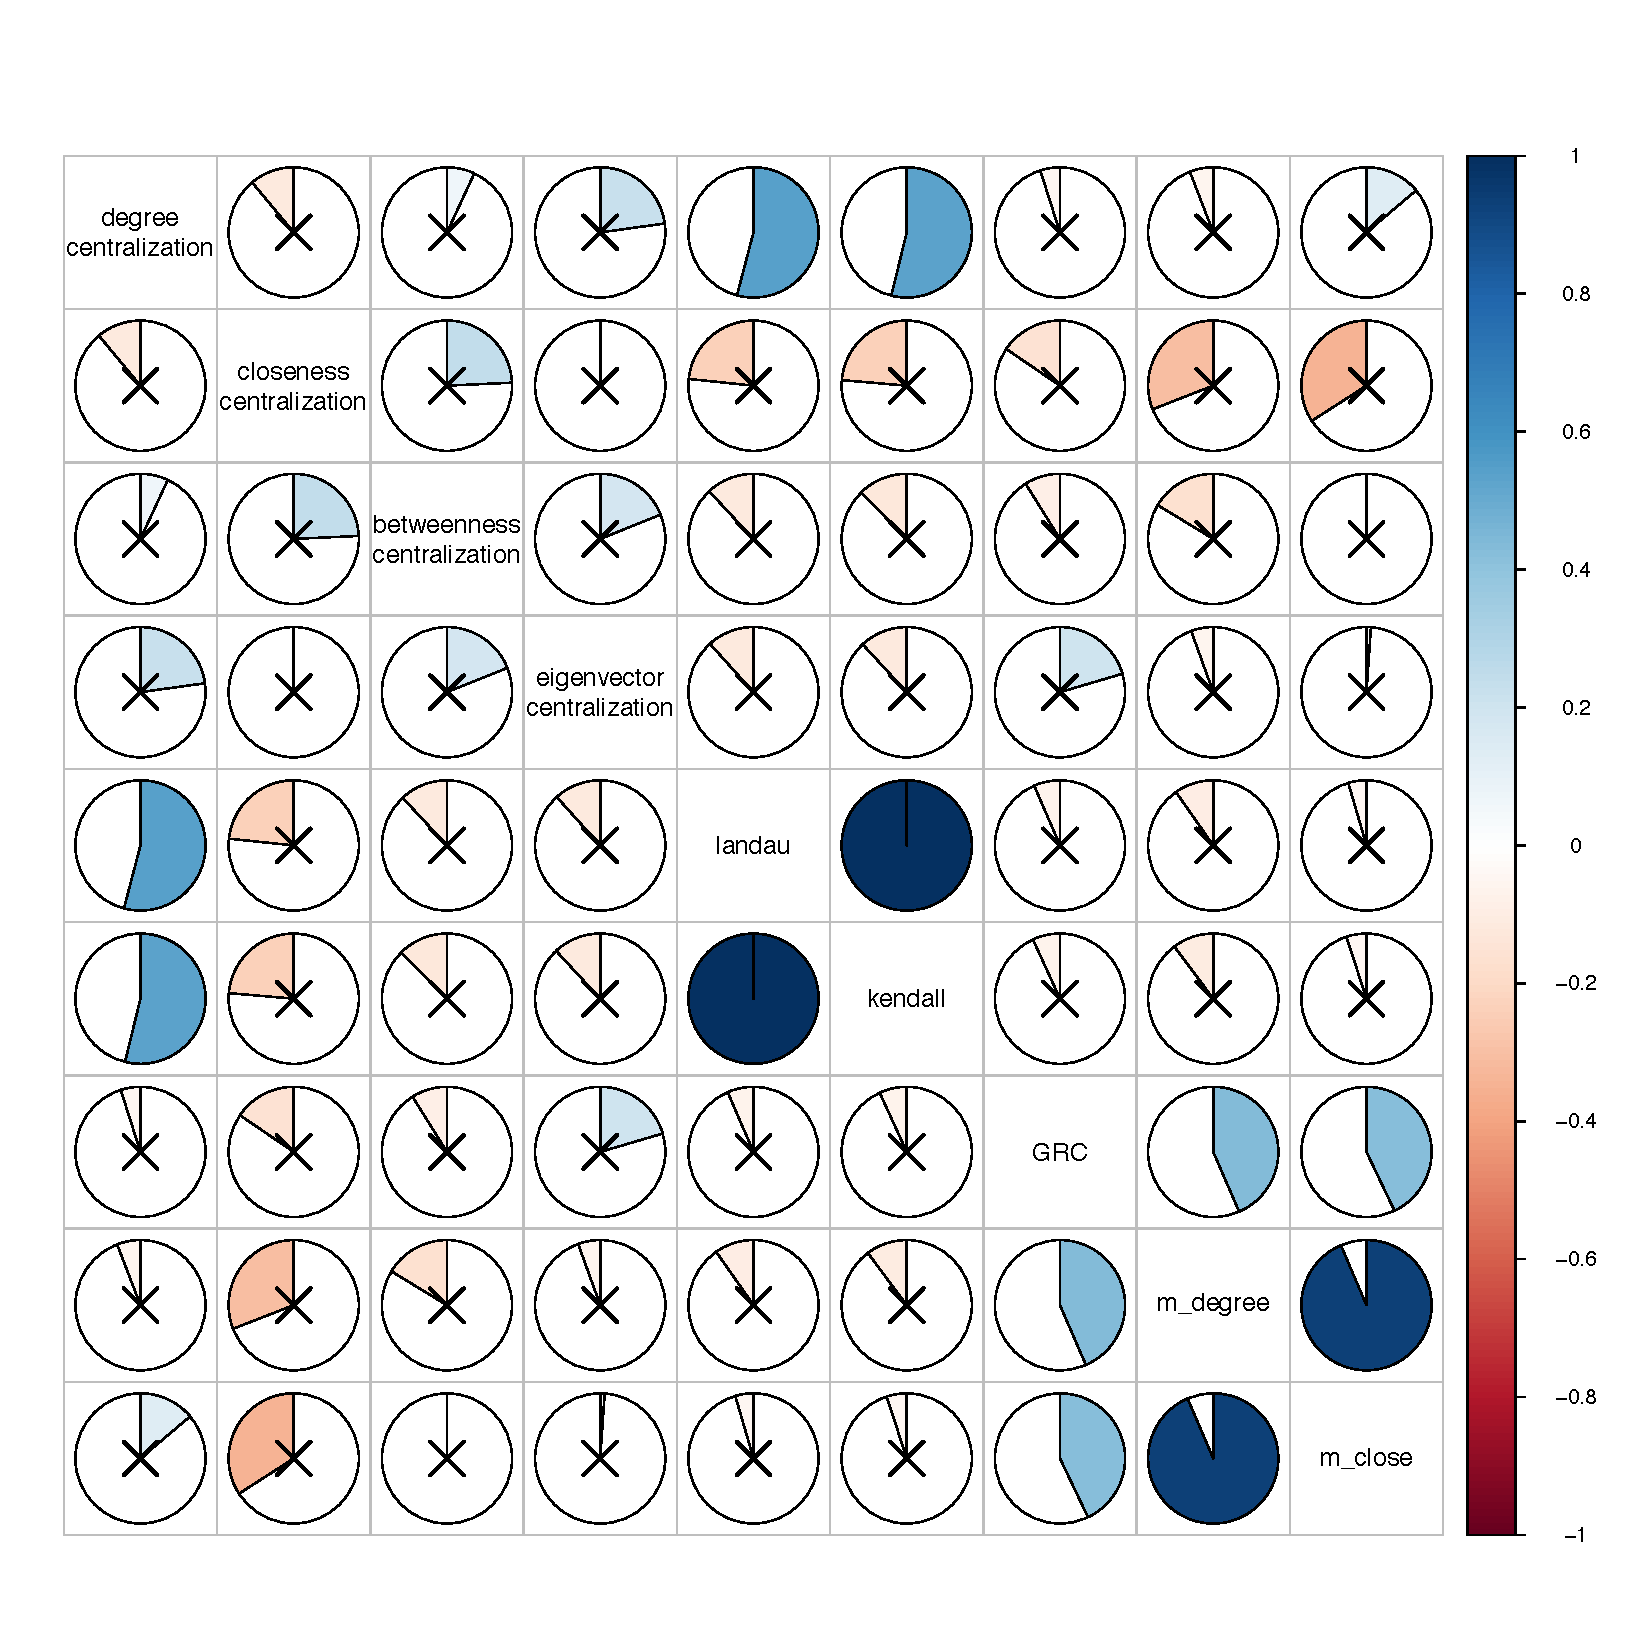
\includegraphics[width = 0.98\textwidth]{./images/Global_Measure_Correlations_with_Tests.pdf}
\end{center}
\end{figure}

Perhaps surprisingly, the rest of the correlations depicted in Figure \ref{fig:measure correlations} are quite small and statistically insignificant, indicating that if all of these measures are valid, they are capturing different dimensions of hierarchy in a network. Figure \ref{fig:pairs plots} provides a full set of pairs plots between all measures, with points for each network colored by the type of network. This finding suggests that either there are multiple dimensions to hierarchy in a network \cite{Corominas-Murtra2013}, some of these measures do not measure hierarchy, or some combination of both. To investigate this finding further, we perform several statistical and qualitative comparisons between these measures in Section \ref{sec:analysis}.

% \subsection{Statistical Measures of Network Hierarchy}
%
% \begin{enumerate}
% 	\item Control Centrality in a weighted and directed graph, defined by \cite{Liu12}, identifies the minimum number of nodes need to drive an entire network to a given final state. Consider a directed, weighted network:
% 	$$
% 	\bm{x}(t) = \bm{Ax}(t) + \bm{Bu}(t)
% 	$$
% 	which is the state of each node at time t, and also denoted as \begin{math}(\bm{A},\bm{B})\end{math}. The components of this controllability matrix are: $\bm{A}\in \mathbb{R}^{N\times N}$, where each element gives the strength that node $j$ can affect node $i$; and $\bm{B}\in\mathbb{R}^{N\times M}$, where each element is the strength between the input signal $u_{j}(t)$ and node $i$, and M contains independent signals imposed by an outside controller. Defining $\bm{C} = (\bm{A}$,$\bm{B})$, the control centr...(line truncated)...
% 	$$
% 	C_{c}(i) \equiv rank_{g}(\bm{C}^{i})
% 	$$
%
% 	\item For social networks, \cite{online} defines hierarchy $h(G)\in[0,1]$ from inferred nodal rankings $r(v)$. Mathematically, it is defined as:
% 	$$
% 	h(G)=1-\frac{1}{m}A(G),
% 	$$
% 	where $A(G)=\sum_{(v_i,v_j)\in E} {max(r(v_i)-r(v_j)+1,0}$ is the total `agony'. Since the rankings are not known, they are found by minimizing the total agony over all possible rankings $r$.
%
% 	\end{enumerate}



% \begin{enumerate}
	% \item Landau's $h\in[0,1]$ is used to compare a directed network to a perfect linear hierarchy \cite{landau}. Let $S_i$ be the row sum for each node, then:
	% 	$$
	% 	h=\frac{12}{N^3-N}\sum_{i=1}^{N}{[S_i-\frac{N-1}{2}]^{2}}
	% 	$$
	% \item Kendall's $K\in[0,1]$ like Landau's $h$ was designed to compare a directed network to a perfect linear hierarchy \cite{kendall}. Let $d$ be the number of cyclic triads defined as: $d=\frac{N(N-1)(2N-1)}{12}-\frac{1}{2}\sum{S_i^2}$. Then:
	% 	$$
	% 	K=1-\frac{d}{d_{max}},
	% 	$$
	% 	where $d_{max} = \left\{ \begin{array}{rl}
	% 	\frac{1}{24}(N^3-N)&\mbox{ if $N$ is odd} \\
	% 	\frac{1}{24}(N^3-4N)&\mbox{ if $N$ is even}
	% 	\end{array} \right.$
	% \item Global reaching centrality, based on the $m$-reach centrality measure is adapted in \cite{GRC} to be a simple measure of hierarchy for any graph:
% 		$$
% 		GRC=\frac{\sum_{i\in V}{[C_R^{max}-C_R(i)]}}{N-1},
% 		$$
% 		\begin{enumerate}
% 			\item When the graph is unweighted and directed, the $C_R(i)$ is the local reaching centrality defined as the proportion of all nodes in $G$ that can be reached along
% 				outgoing edges from node $i$.
% 			\item When the graph is weighted and directed, the following version for the reaching centrality as defined in \cite{GRC} is used:
% 				$$
% 				C_{R}^{'}(i)=\frac{1}{N-1}\sum_{j: 0<d^{out}_{(i,j)}<\infty}{( \frac{\sum_{k=1}^{d^{out}(i,j)} {w_{i}^{(k)} (j) } }{d^{out}(i,j)} )},
% 				$$
% 				where $d^{out}_{i,j}$ is the length of the directed outgoing path from $v_{i}$ to $v_{j}$ and $w^{(k)}_{i}$ is the weight of the $k$th edge along this path.
% 			\item When the graph is unweighted and undirected, the following version for the reaching centrality as defined by \cite{GRC} is used:
% 				$$
% 				C_{R}^{''}(i)=\frac{1}{N-1}\sum_{j:0<d(i,j)<\infty}{\frac{1}{d(i,j)}}
% 				$$
% 		\end{enumerate}
%
% 	\item Rooted depth in directed networks is defined in \cite{depth}, where a root is a node that has only incoming edges. Let $N_{r}$ be the number of node-root pairs in the network. Then the global root depth is defined as:
% 		$$
% 		D=\frac{1}{N_{r}}\sum_{i=1}^{N_r}{l_{ri}},
% 		$$
% 		where $l$ is the length of the shortest path between root $r$ and node $i$.
	% \item We apply centralization, a method used to calculate a global measure of centrality from local measures, to the following local centrality measures: betweenness, closeness, eigenvector, and degree, all of which are defined in the following section. Centralization is defined as follows for local measures $c_{i}$:
	% $$
	% C=\sum_{i=1}^{N}{(max\{c_{i}\}-c_{i})}
	% $$
% \end{enumerate}

% \subsection{Measures of Hierarchy-Local}
% \begin{enumerate}
	% \item M-reach degree was developed to identify `key' players in a network \cite{key} and is defined for a vertex $v_{i}$ as the number of reachable vertices from $v_{i}.$ If
	% 	$G$ is directed then this reachable vertices must lie along an outgoing path from $v_{i}$. This local measure is the same used for the $GRC$ local measures in \cite{GRC}.
	% \item M-reach closeness was also developed to identify `key' players \cite{key}. It is defined as the M-reach degree weighted by the inverse geodistances. 
	% \item A local version of rooted depth can be found for a graph. Given $r$ roots in a network, the each node has a local root depth equal to the average length of the shortest path between itself and all roots \cite{depth}.
	% \item Betweenness centrality is meant to capture the amount of influence a node has on the information transversed through it \cite{between}. Define $D_{i,j}$ as the number of shortest paths between $v_{i}$ and $v_{j}$ and $D_{i,j}(k)$ as the number of these shortest paths that pass through $v_{k},$ then the betweenness centrality for $v_{k}$ is:
	% 	$$
	% 	\sum_{i\neq k\neq j}{(\frac{D_{i,j}(k)}{D_{i,j}})}
	% 	$$
	% \item Given $d(i,j)$ is the length of the shortest path between $v_{i}$ and $v_{j}$, closeness centrality is measured as
	% 	$$
	% 	\sum_{i\neq j}{(\frac{1}{d(i,j)})}
	% 	$$
	% \item Eigenvector centrality is meant to give weight to nodes that are connected to nodes that are most central in the network \cite{eigen}. Defining the graphs adjacency matrix
	% 	as $A$ and the vector of local eigenvector centrality scores as $c=\{c({v_{1}}),...,c(v_{V})\}$ we have to solve the following equation:
	% 	$$
	% 		A c=\lambda c
	% 	$$
	% \item Degree centrality for $v_{i}$ is simply the number of outgoing edges it has.
% \end{enumerate}

% \subsection{Discussion of Measures}
% For the global measures, both Landau's $h$ and Kendall's $K$ have mostly been used to determine so called pecking order among animals \cite{animals}. Due to their ability to capture the degree to which a network is linearly hierarchical, we expect these measures to perform similarly. We also expect all three centralization scores to perform the same. We note that rooted depth is only defined for graphs with at least one root. If there is no root the measure classifies the network as having no hierarchy. For the local measures, we expect M-reach degree and degree to be correlated since M-reach degree was defined based on degree centralization. Similarly we expect M-reach closeness to be correlated to closeness.


















	
	
\section{Data}
\label{sec:data}
We refer to three main sources for our data. The first set of networks, County Managers, contains information on email communications between 17 county managers and their staff. They are categorized as communication networks. Our second set of networks contains information on 17 bills in congress and are classified as co-sponsorship networks. Our final source of data contains all networks found within UCINET. After removing $11$ networks that were undirected, two-mode, or extreme outliers, we were left with a total of $136$ networks. Of the $102$ UCINET datasets included in our analysis, $33$ did not have a classification. Since there are no clear guidelines on how UCINET defined types for each dataset, the accurate categorization of these $33$ networks did not appear viable. These datasets are classified as unknown networks. Descriptive statistics for each of the nine types of networks we consider in this study are provided in Table \ref{tab:descriptive stats by type}.  
%A list of references for the network datasets used in this study can be found in \ref{sec:dataset references}.

% latex table generated in R 3.2.2 by xtable 1.8-0 package
% Sun Dec  6 14:21:01 2015
\begin{table}[ht]
\centering
\caption{\label{tab:descriptive stats by type} Network Descriptive statistics for all 136 networks in our sample, aggregated by the network type. All columns are averages over networks of that type.}
\begin{tabular}{lrrrrr}
  \toprule
 \textbf{Type} & \textbf{\# of Networks} & \textbf{Nodes} & \textbf{Edges} & \textbf{Density} & \textbf{Clustering Coefficient} \\ 
  \midrule
\emph{communication} & 20 & 25.40 & 1764.25 & 2.87 & 0.55 \\ 
  \emph{cosponsorship} & 18 & 101.22 & 13358.89 & 1.32 & 0.79 \\ 
  \emph{co-membership} & 2 & 21.50 & 22.50 & 0.05 & 0.07 \\ 
  \emph{interaction} & 40 & 23.07 & 1944.95 & 1.99 & 0.59 \\ 
  \emph{unknown} & 33 & 38.70 & 445.36 & 0.38 & 0.43 \\ 
  \emph{friendship} & 6 & 29.83 & 92.00 & 0.12 & 0.35 \\ 
  \emph{affect} & 11 & 17.64 & 95.18 & 0.32 & 0.33 \\ 
  \emph{terrorism} & 1 & 63.00 & 308.00 & 0.08 & 0.36 \\ 
  \emph{trade} & 5 & 24.00 & 285.60 & 0.52 & 0.73 \\ 
   \bottomrule
\end{tabular}
\end{table}

Before fitting any of the hierarchy measures on these real datasets, we want to make sure that the measures are invariant to the size of the network. We simulate $7500$ Barbasi-Albert (BA), $6000$ Tree-Structured (TR), and $4500$ Erdos-Renyi (ER) datasets, where one third of each type has $50$ nodes, a third has $200$, and the last third has $500$. We are also curious to see how the hierarchy measures perform while altering the parameters of these datasets. For the BA datasets, we set the preferential treatment parameter to $p=0.5, 1, 2, 5, 10$. We set the number of children parameter in the TR datasets to be $c=2, 5, 10, 50$, and the probability of forming and edge in the ER datasets to $d=0.05, 0.1, 0.2$. Figures can be found in Appendix C, which illustrate our findings. For the BA networks, we notice that Kendall and Landau's measures do not change as $p$ increases. We note that all other measures except for degree and closeness decrease as $p$ increases. For TR networks,   
	
% Among the network datasets we are exploring, they are already or mostly in usable format. As we're navigating through our theoretical conception of hierarchy in network, we are ruling out the use of the karate club, dolphin, football, etc. datasets because we want to be able to analyze datasets where the networks are more interesting or theoretically-relevant. In this way, there are a couple of systems that might be useful. The first is a network of cooperation among militant groups, which encompasses joint exercises, mergers, and splits among militant groups: http://web.stanford.edu/group/mappingmilitants/cgi-bin/. This may interesting for us for a few reasons: (1) there is no de jure hierarchical structure (i.e., no formally-recognized chain of command or sovereignty); (2) militant groups face a classic collective action problem, and thus we can expect the dynamics Mann describes to hold; and (3) most theories of conflict would predict no hierarchy to occur in this system. An interesting system to compare this to would be military actions in Vietnam: http://tinyurl.com/pwofooy. The nodes here would be military units, and the edges are participation in the same battle. Of course, the main issue with this dataset is that it's undirected, which we've noted may be difficult to conceptualize within a hierarchy framework. We're focusing on conflict datasets because many of the theoretical definitions define hierarchy as essentially about outcomes—i.e., the ability of particular nodes to control the actions and behaviors of subordinate nodes.
%
%  We may also use manager network data where each organization has a ``county manager" who is theoretically in charge of the rest of the actors, providing an opportunity to determine if the methods we employ capture a plausible hierarchical structure. We are still exploring this and other datasets though.





\section{Analysis}
\label{sec:analysis}

PCA component eigenvalues are illustrated in Figure \ref{fig:PCA variacnes}. A graphical comparison of components one and two is provided in \ref{fig:1 and 2}. A graphical comparison of components one and three is provided in \ref{fig:1 and 3}. A graphical comparison of components two and three is provided in \ref{fig:2 and 3}.



\begin{figure}
\begin{center}
	\caption{\label{fig:PCA variacnes} Eigenvalues for 9 largest principle components in our analysis indicate that we should examine the first three components, which all have eigenvalues greater than one.}
		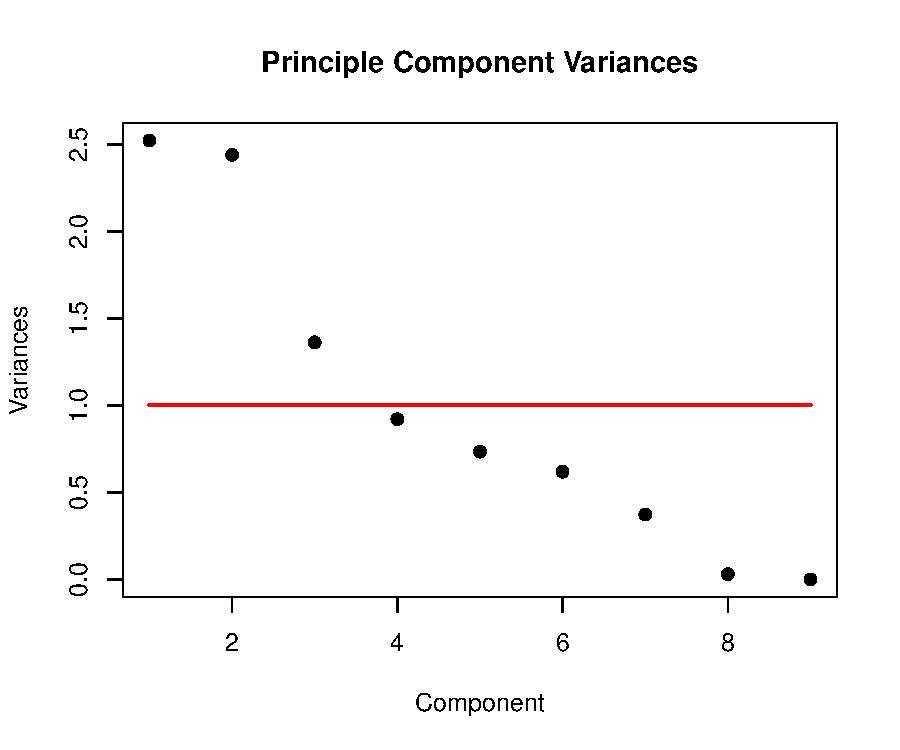
\includegraphics[width = 0.5\textwidth]{./images/Observed_PCA_Component_Varinces.pdf}
\end{center}
\end{figure}

\begin{figure}
\begin{center}
	\caption{\label{fig:1 and 2} Principle components plot for components one and two.}
		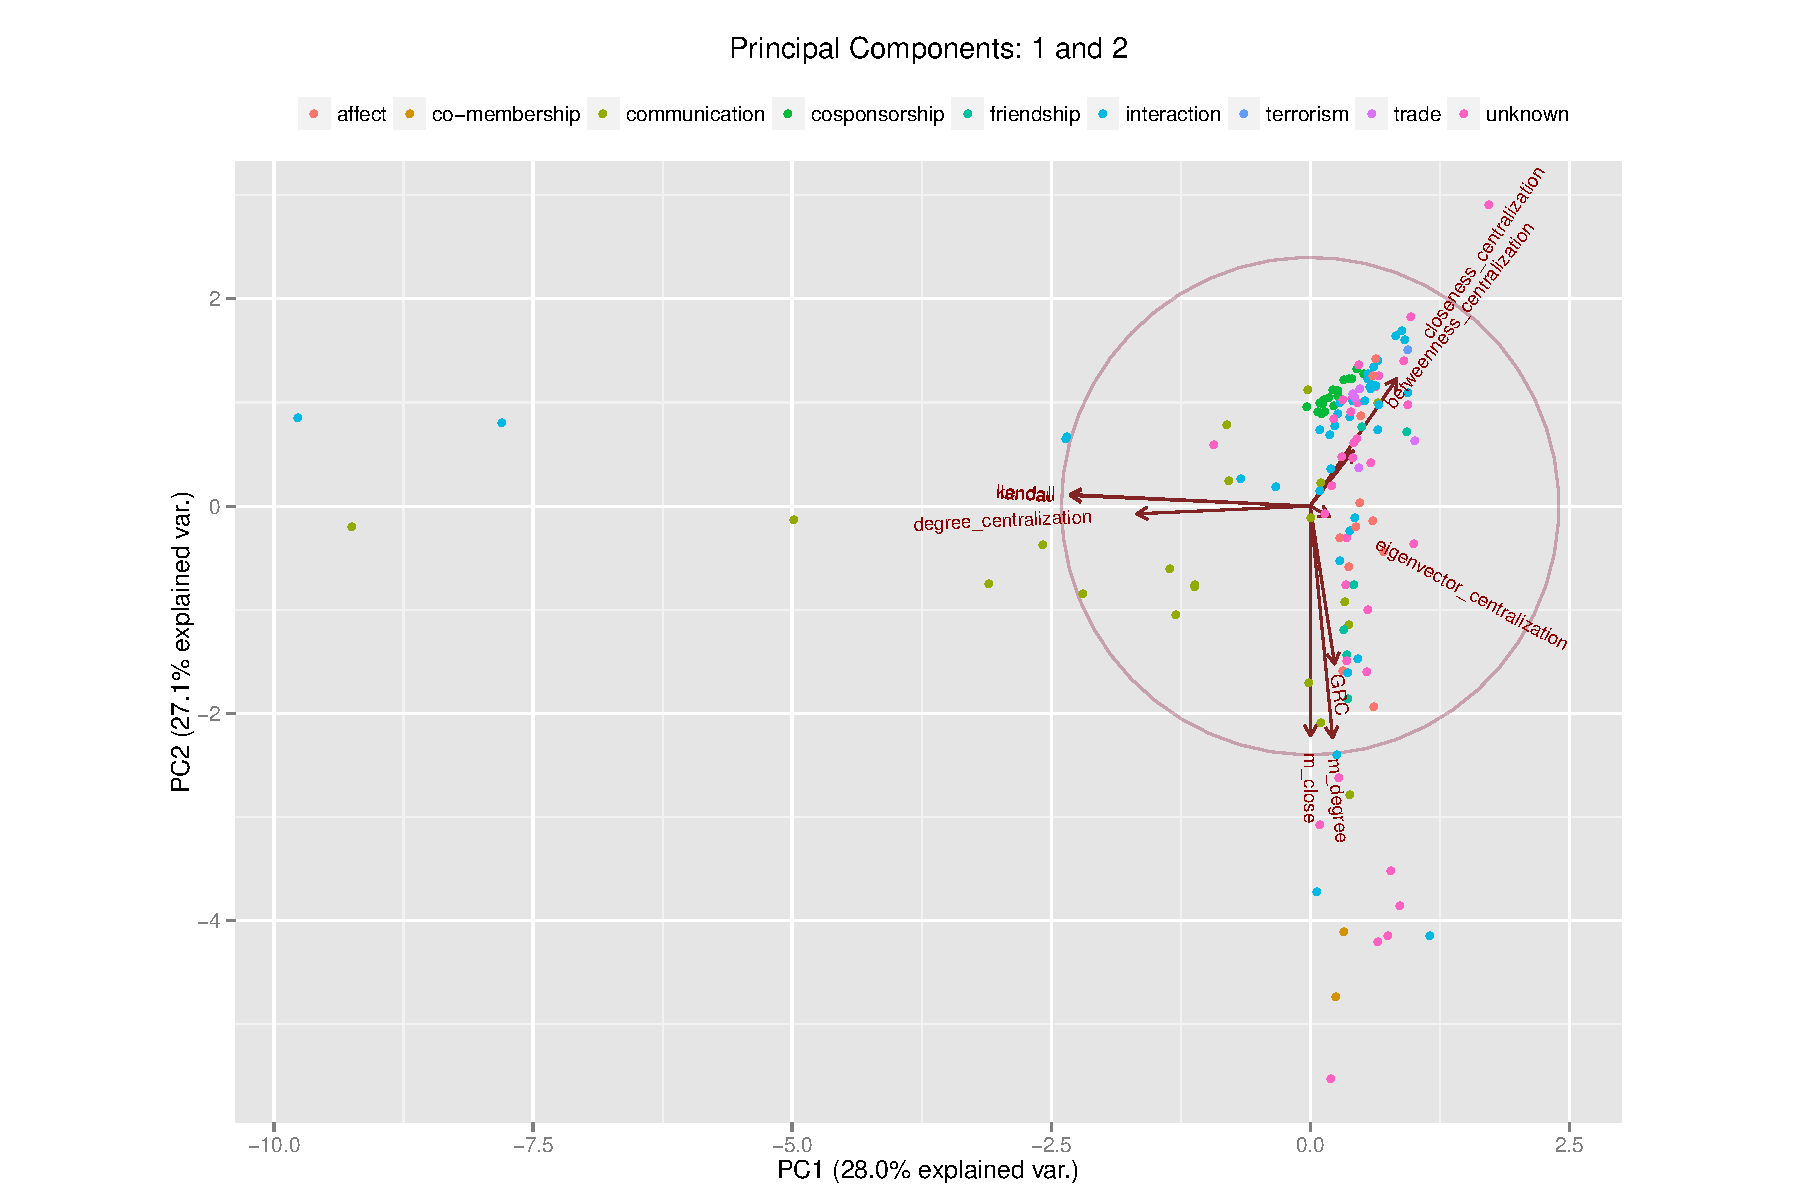
\includegraphics[width = 0.98\textwidth]{./images/Observed_PCA_Components1_2.pdf}
\end{center}
\end{figure}

\begin{figure}
\begin{center}
	\caption{\label{fig:1 and 3} Principle components plot for components one and three.}
		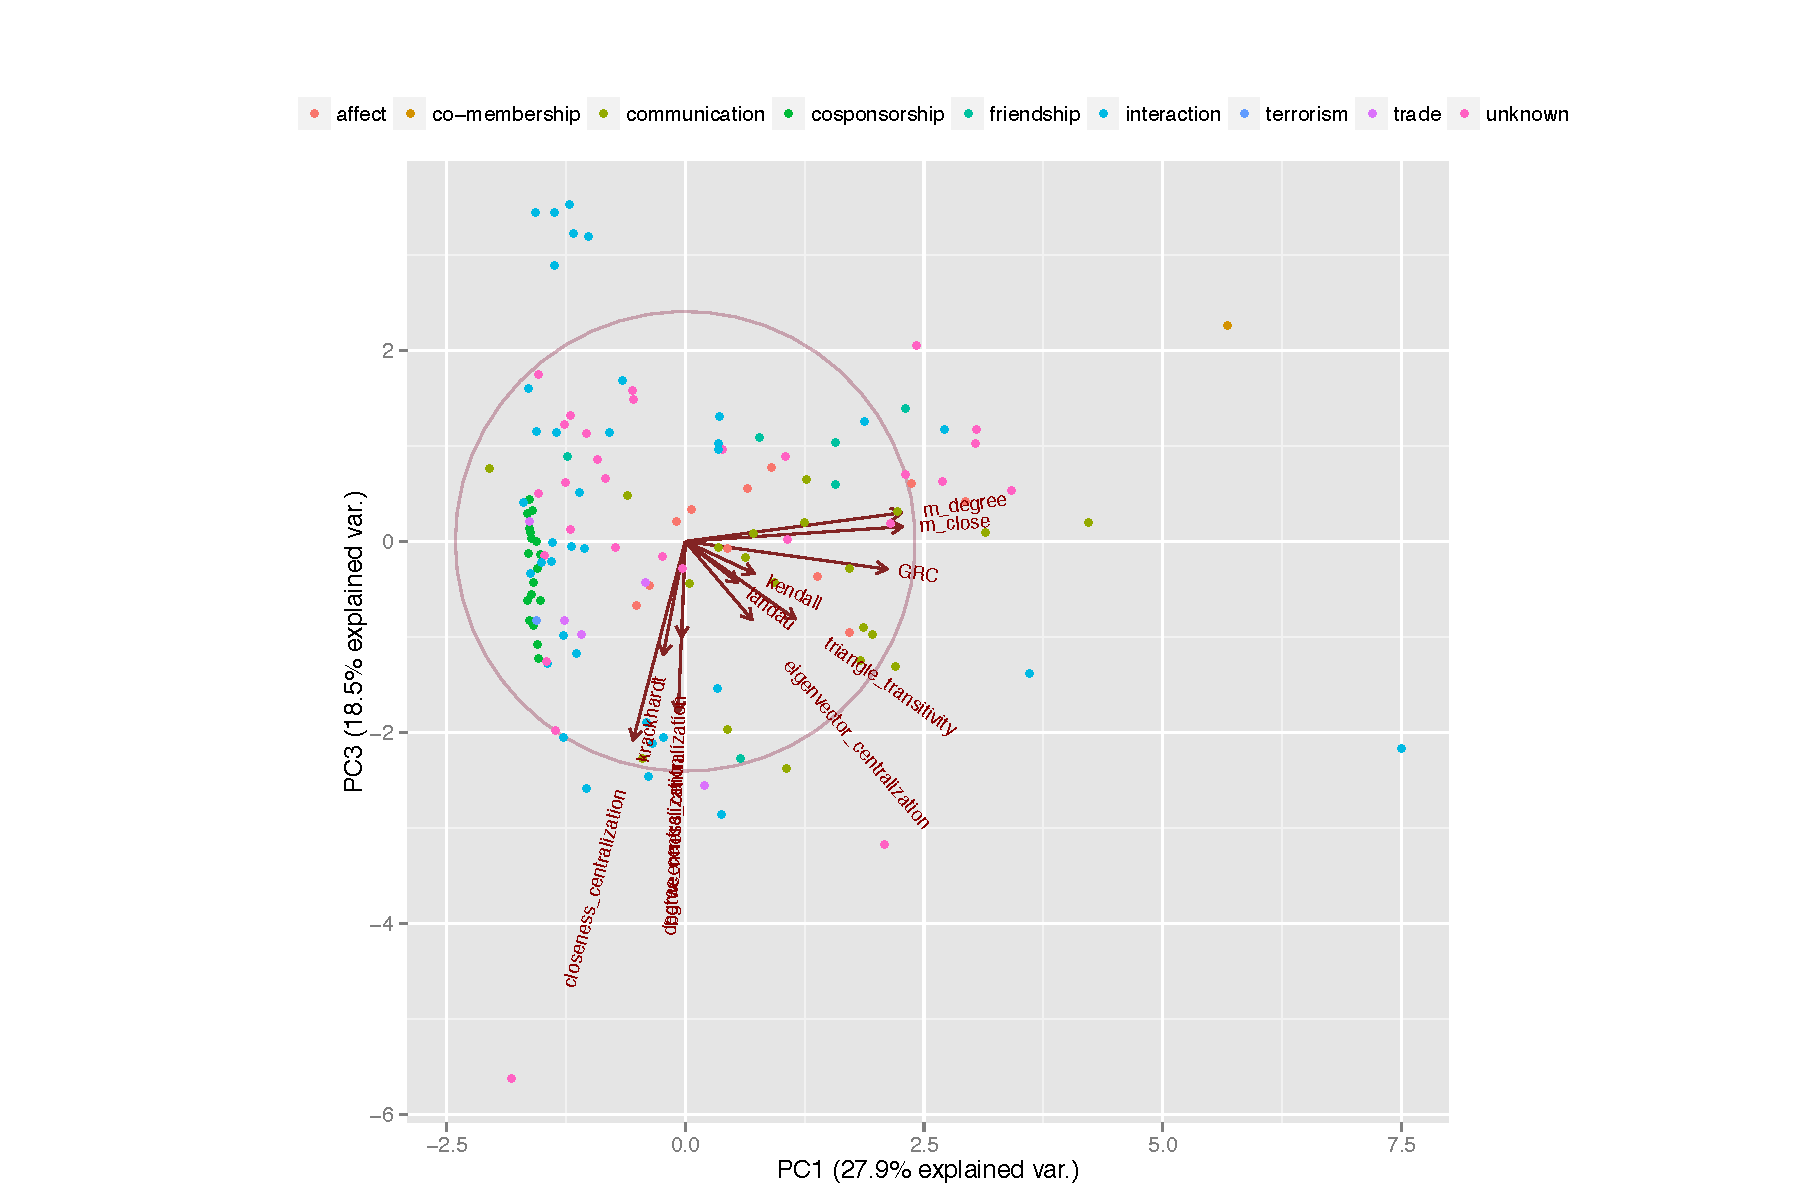
\includegraphics[width = 0.98\textwidth]{./images/Observed_PCA_Components1_3.pdf}
\end{center}
\end{figure}

\begin{figure}
\begin{center}
	\caption{\label{fig:2 and 3} Principle components plot for components two and three.}
		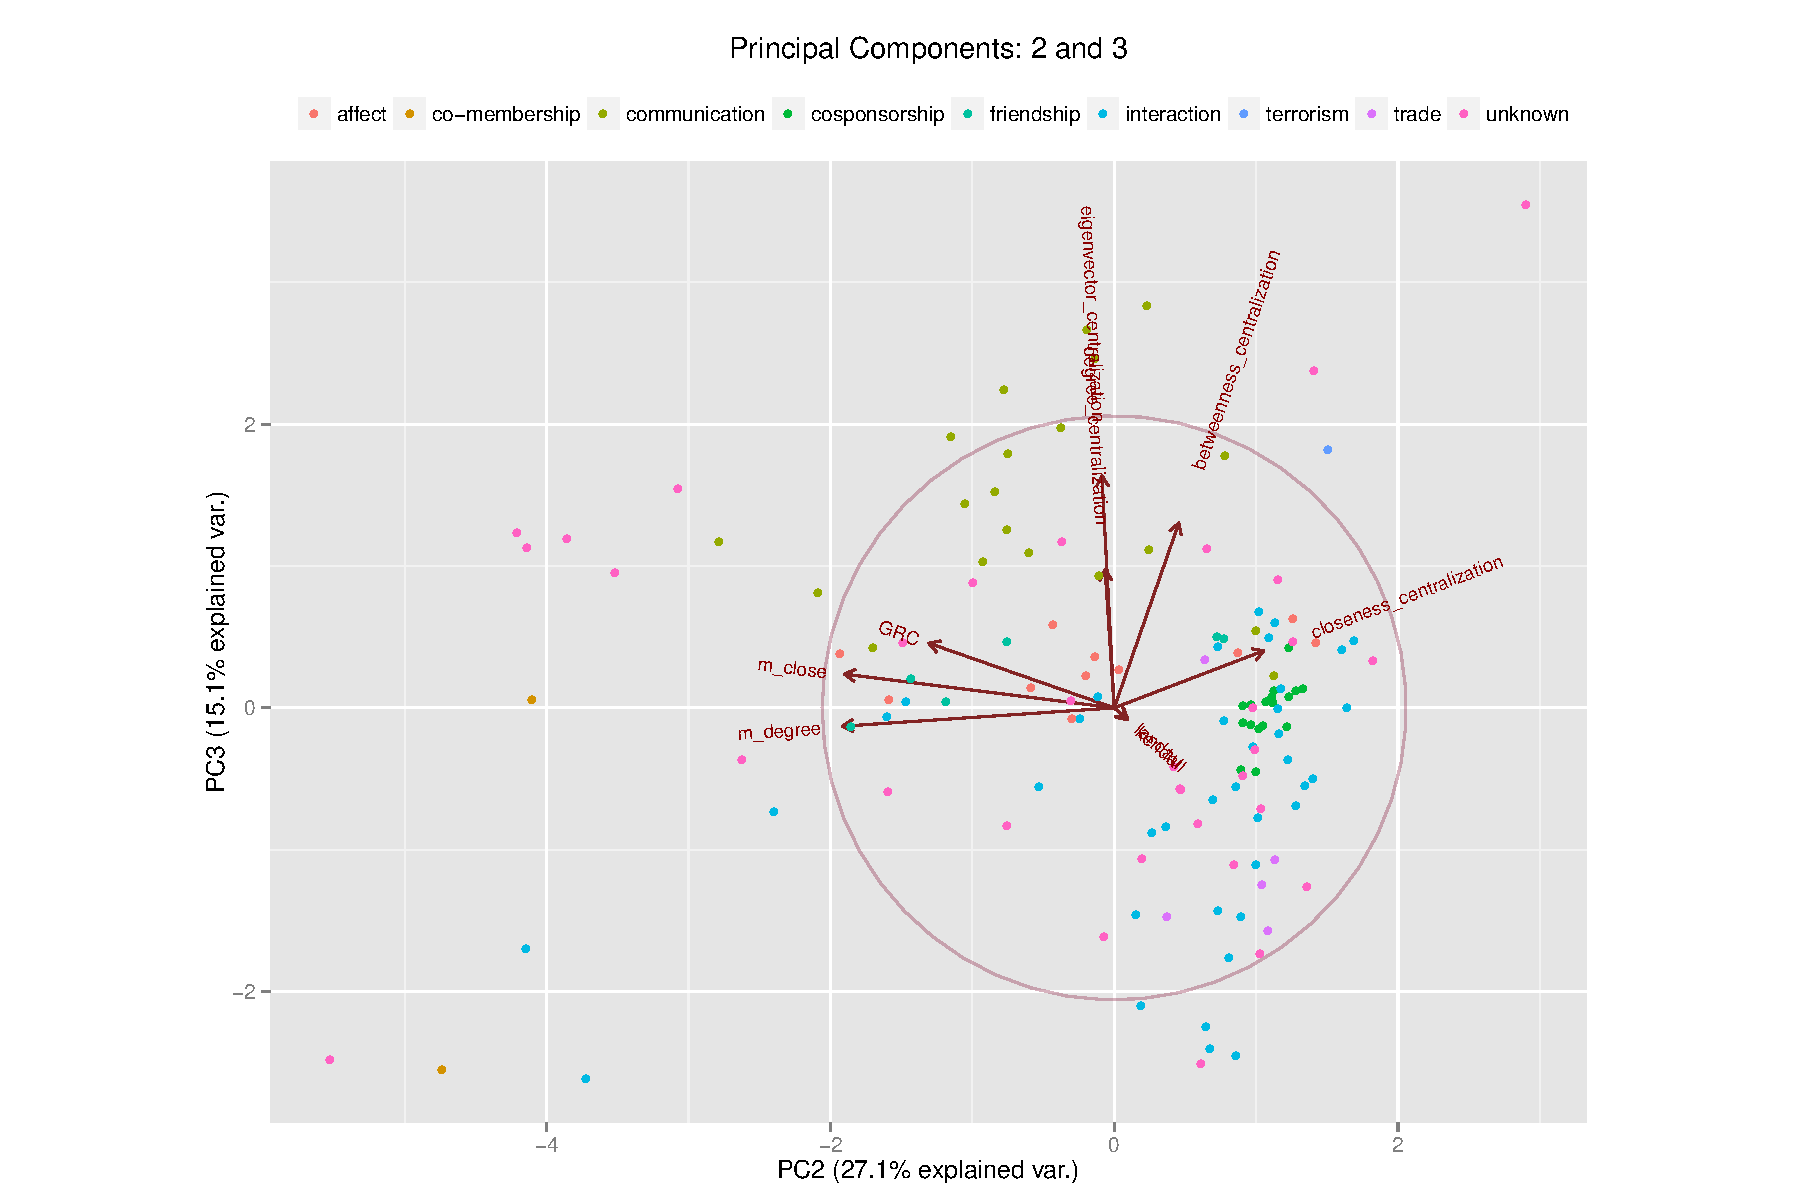
\includegraphics[width = 0.98\textwidth]{./images/Observed_PCA_Components2_3.pdf}
\end{center}
\end{figure}


% latex table generated in R 3.2.2 by xtable 1.8-0 package
% Fri Dec 11 16:43:36 2015
\begin{table}[ht]
\centering
\begin{tabular}{rr}
  \hline
 & average\_rank \\ 
  \hline
degree\_centrality & 0.75 \\ 
  closeness\_centrality & 0.82 \\ 
  betweenness\_centrality & 0.78 \\ 
  eigenvector\_centrality & 0.78 \\ 
  m\_degree & 0.81 \\ 
  m\_close & 0.63 \\ 
  GRC & 0.36 \\ 
  D\_root & 0.86 \\ 
   \hline
\end{tabular}
\end{table}

% 	The analytical portion of the problem will be conducted in R, which is known by all members of the group. We will be using both statistical and mathematical methods of quantifying and/or measuring hierarchy. We will focus on methods that have already been developed, published, and implemented in R, or are can easily be implemented by one of the group members. If time permits, we may try to develop or suggest directions for future development of our own statistical models and/or mathematical measurements. Each member of the group will be responsible for at least one method.
%
% The statistical methods we will be looking into include hierarchical exponential graph models in the R package hergm. This package also includes hierarchical stochastic block models. Unlike fitting network data with exponential random graph models (ERGMs), hierarchical ERGMs focus on inducing local dependencies. Next, we will focus on latent space models, which can be fit in R using the latentnet package in the statnet suite of packages. For both the latent space and ERGM models, Bayesian inferential analysis can be conducted using the Bergm, VBLPCM, and lvm4net packages in R. We note that whenever fitting network data there is always the chance for computational timing and accuracy issues to come up. We have chosen a number of datasets for the purposes of capturing several types of hierarchies, but also so that we may have a few that are easily fit in R. Lastly, we will focus on mathematical measures of hierarchy. These measures primarily stem from graph theory, and can be easily programed by ourselves in R. The measurements include the Global Reach Centrality (GRC), Triangle Transitivity, Kendall's K, and Landau's lambda.



\section{Conclusions}

\bibliographystyle{elsarticle-num}
\bibliography{library}

%% Authors are advised to use a BibTeX database file for their reference list.
%% The provided style file elsarticle-num.bst formats references in the required Procedia style

%% For references without a BibTeX database:

% \begin{thebibliography}{00}
\begin{thebibliography}{9}
	\bibitem{key} 
	An,W. (2015),
	``Multilevel Meta Network Analysis with Application to Studying Network Dynamics of Network Interventions." \textit{Social Networks} 43: 48-56.
	
	\bibitem{eigen} 
	Bonacich, P. (1972),
	``Factoring and Weighting Approaches to Status Scores and Clique Identification." 
	\textit{Journal of Mathematical Sociology} 2: 113-120.
	
	\bibitem{monks}
	Breiger, R., Boorman, S., and Arabie, P. (1975),
	``An algorithm for clustering relational data with applications to social network analysis and comparison with multidimensional scaling."
	\textit{Journal of Mathematical Psychology} 12.
	
	\bibitem{libi}
	Brozovsky, L. and Petricek, V. (2007),
	``Recommender system for online dating service."
	\textit{Proc. Znalosti} 29-40.
	
	\bibitem{docs}
	Coleman, J., Katz, E., and Menzel, H. (1957),
	``The diffusion of an innovation among physicians."
	\textit{Sociometry} 253-270.
	
	\bibitem{HS}
	Coleman, J. (1973),
	``Introduction to mathematical sociology."
	\textit{London Free Press Glencoe}.
	
	\bibitem{Corominas-Murtra2013}
	Corominas-Murtra, B., Goni, J., Sole, R. V, \& Rodríguez-Caso, C. (2013). ``On the origins of hierarchy in complex networks''. \emph{Proceedings of the National Academy of Sciences of the United States of America}, 110(33), 13316–21. \href{http://doi.org/10.1073/pnas.1300832110}{http://doi.org/10.1073/pnas.1300832110}
	
	\bibitem{between} 
	Freeman, L. (1977),
	``A set of Measures of Centrality Based on Betweenness." 
	\textit{Sociometry} 40: 1, 35-41.
	
	\bibitem{Res}
	Freeman, L., Webster, C., and Kirke, D. (1998),
	``Exploring social structure using dynamic three--dimensional color images."
	\textit{Social Networks} 20: 2, 109-118.
	
	\bibitem{friendster}
	Friendster network dataset - KONECT, May 2015.
	
	\bibitem{URV}
	Guimera, R., Danon, L., Diaz-Guilera, A., Giralt, F., and Arenas, A. (2003),
	``Self--similar community structure in a network of human interactions."
	\textit{Phys. Rev. E.} 68: 6.
	
	\bibitem{online} 
	Gupte, M., Shankar, P., Li, J., Muthukrishnan, S., and Iftode, L. (2011),
	``Finding Hierarchy in Directed Online Social Networks." 
	\textit{International World Wide Web Conference Committee (IW3C2)}.
	
	\bibitem{Digg}
	Hogg, T. and Lerman, K. (2012),
	``Social dynamics of Digg."
	\textit{EPJ Data Science} 1, 5.
	
	\bibitem{kendall} 
	Kendall, M. and Babington Smith B. (1940),
	``On the Method of Paired Comparisons." 
	\textit{Biometrika} 31: 324-345.
	
	\bibitem{landau} 
	Landau, H. G. (1951),
	``On Dominance Relations and the Structure of Animal Societies:  Effect of inherent characteristics." 
	\textit{Bulletin of Mathematical Biology} 13: 245-262.

	\bibitem{EU}
	Leskovec, J., Kleinber, J., and Faloutsos, C. (2007),
	``Graph Evolution: Densification and Shrinking Diameters."
	\textit{ACM Transactions on Knowledge Discovery from Data (ACM TKDD)} 1: 1.

	\bibitem{livejournal}
	Leskovec, J., Lang, K., Dasgupta, A., and Mahoney, M. (2009),
	``Community Structure in Large Networks: Natural Cluster Sizes and the Absence of Large Well-Defined Clusters."
	\textit{Internet Mathematics} 6: 1, 29-123.

	\bibitem{wiki}
	Leskovec, J., Huttenlocher, D., and Kleinberg, J. (2010),
	``Predicting Positive and Negative Links in Online Social Networks."
	
	\bibitem{linux}
	Linux kernel mailing list replies network dataset - KONECT, May 2015.

	\bibitem{Liu12}
	Liu, Y., Slotine, J., and Barab{\'a}si, A (2012),
	``Control centrality and hierarchical structure in complex networks."
	\textit{Plos ONE:} 7: 9.
	
	\bibitem{mann}
	Mann, Michael. (1986), ``Chapter 1: Societies as organized power networks."
	\textit{The Sources of Social Power, Volume 1, A history of power from the beginning to AD 1760}. Cambridge University Press: 1-33.
	
	\bibitem{facebook}
	McAuley, J. and Leskovec, J. (2012),
	``Learning to Discover Social Circles in Ego Networks."	\textit{NIPS}.
	
	\bibitem{manufacturing}
	Michalski, R., Palus, S., and Kazienko, P. (2011),
	``Matching organizational structure and social network extracted from email communication."
	Lecture Notes in Business Information Processing: 87, 196-206.
	
	\bibitem{youtube}
	Mislove, A., Marcon, M., Gummadi, K., Druschel, P., and Bhattacharjee, B. (2007),
	``Measurement and analysis of online social networks."
	\textit{Proc. Internet Measurement Conference}.
	
	\bibitem{GRC} 
	Mones, E., Vicsek, L., and Vicsek, T. (2012),
	``Hierarchy Measure for Complex Networks." 
	\textit{Plos ONE} 7: 3, 1-10.	
	
	\bibitem{AdHealth}
	Moody, J. (2001),
	``Peer influence groups: Identifying dense clusters in large networks."
	\textit{Social Networks} 23: 4, 261-283.
	
	\bibitem{irvine}
	Opsahl, T. and Panzarasa, P. (2009),
	``Clustering in weighted networks."
	\textit{Social Networks} 31: 2, 155-163.
	
	\bibitem{cite}
	Prosper loans network dataset - KONECT, May 2015.
	
	\bibitem{epinions}
	Richardson, M., Agrawal, R., and Domingos, P. (2003),
	``Trust Management for the Semantic Web." \textit{ISWC}.
	
	\bibitem{Taro}
	Schwimmer, E. (1973),
	``Exchange in the Social Structure of the Orokaiva: Traditional and Emergent Ideologies in the Northern District of Papua." \textit{St. Martin's Press}.
	
	\bibitem{animals} 
	Shizuka, D. and McDonald, D. B. (2012),
	``A social network perspective on measurements of dominance hierarchies." 
	\textit{Animal Behavior} 83: 925-934.
	
	\bibitem{depth} 
	Suchecki, K. and Holyst, J. (2013),
	``Hierarchy depth in directed networks." 
	\textit{Physica A} arXiv:1303-2085.
	
	\bibitem{pokec}
	Takac, L. and Zabovsky, M. (2012),
	``Data Analysis in Public Social Networks."
	International Scientific Conference \& International Workshop Present Day Trends of Innovations, Lomza, Poland.
	
	\bibitem{Dutch}
	Van de Bunt, G., Van Deuijn, M., and Snijders, T. (1999),
	``Friendship networks through time: An actor-oriented dynamic statistical network model."
	\textit{Computational and Mathematical Organization Theory} 5: 2, 167-192.
	
	\bibitem{Wasserman1994}
	Wasserman, S., \& Faust, K. (1994). ``Social Network Analysis: Methods and Applications''. (M. Granovetter, Ed.)\emph{Social Networks (Vol. 8)}. Cambridge University Press. \href{http://doi.org/10.2307/2077235}{http://doi.org/10.2307/2077235}
	
	\bibitem{sevies}
	Watts, D. and Strogatz, S. (1998),
	``Collective dynamics of `small world' networks."
	\textit{Nature} 393: 1, 440-442.
	
	\bibitem{wiki2}
	West, R., Paskov, H., Leskovec, J., and Potts, C. (2014),
	``Exploiting Social Network Structure for Person-to-Person Sentiment Analysis."
	\textit{Transactions of the Association for Computational Linguistics} 2: 297-310.
	
	\bibitem{Yitzhaki1979}
	Yitzhaki, S.. (1979), ``Relative deprivation and the Gini coefficient." \emph{The quarterly journal of economics} 321-324.

	


    
    
    
\end{thebibliography}
%% \bibitem must have the following form:
%%   \bibitem{key}...
%%

% \bibitem{}

% \end{thebibliography}

\newpage
\appendix


\section{Measure Pairs Plots}
\label{sec:pairs plots}

\begin{figure}[htp]
\begin{center}
	\caption{\label{fig:pairs plots} Pairs plots between nine network hierarchy measures calculated on 136 networks. Points are colored according to network type, with the following color codings: \textbf{affect} = black,         \textbf{co-membership} = yellow,  \textbf{communication} = red, \textbf{bill cosponsorship} = orange, \textbf{friendship} = green,  \textbf{interaction} = blue, \textbf{terrorism} = pink, \textbf{trade} = maroon, and all networks for which the type was \textbf{unknown} were collored light brown.}
		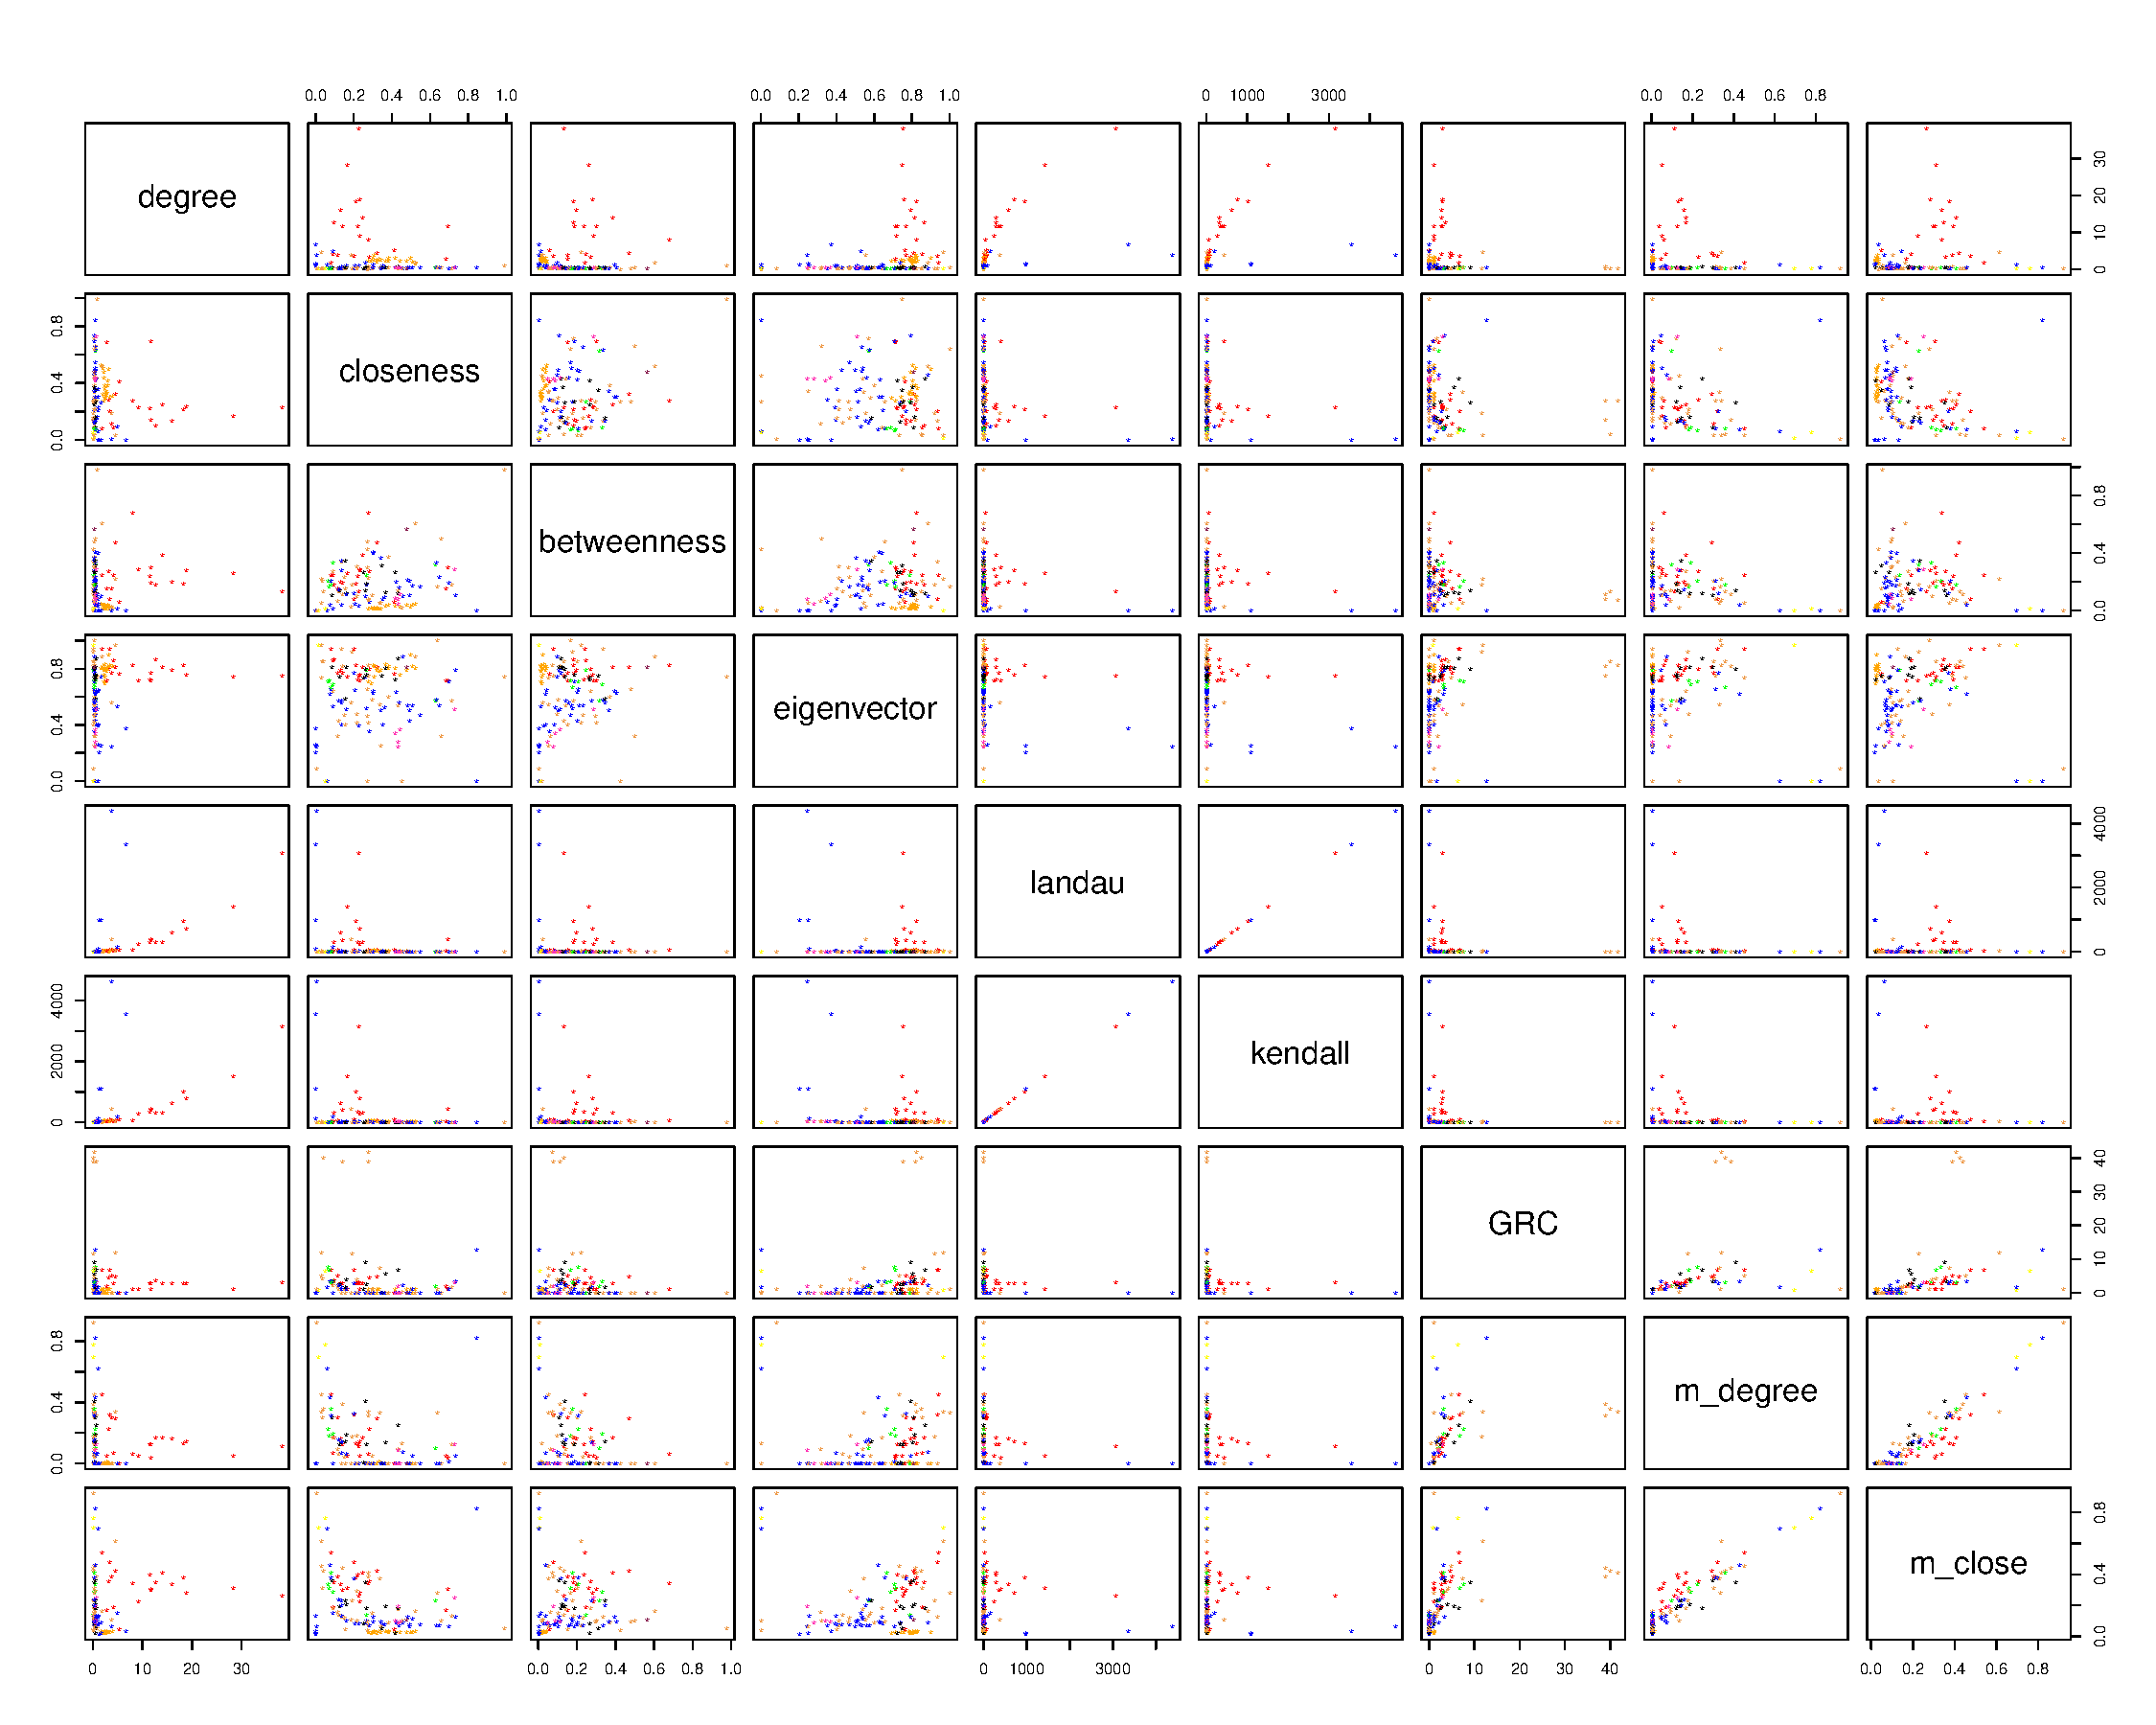
\includegraphics[width = 0.98\textwidth]{./images/Global_Measure_Pairs_Plots.pdf}
\end{center}
\end{figure}


\section{Dataset References}
\label{sec:dataset references}

\begin{enumerate}


    	
    	\item Adolescent Health: survey asked students to list 5 male and female friends. \cite{AdHealth}
    	
    	\item Residence Hall: friendships between 217 students in Australian National University. \cite{Res}
    	
    	\item Taro Exchange: gift--giving relationships between households in a Papaun village. \cite{Taro}
    	
    	\item Highschool: friendship relationship between boys at a small Indiana high school in 1957-1958. \cite{HS}
    	
    	\item Dutch College: friendships between 32 university freshmen. \cite{Dutch}
    	
    	\item Monks: preference ratings between monks in a cloister during a crisis. \cite{monks}
    	
    	\item Physicians: innovation spread between 246 physicians in Illinois. \cite{docs}
    	
    	\item Seventh graders: activity specific proximity rankings for 29 middle school students in Victoria \cite{sevies}.
    
    \item Prosper loans: loans between users of prosper.com \cite{prosper}.
    
    \item Libimseti.cz: likes between users on a Czech dataing site \cite{libi}.
    
    %\item Friendster: friendship adds on the online site Friendster \cite{friendster}.
    
    \item Digg: friendships on Digg \cite{digg}.
    
    \item Youtube: connections between Youtube users \cite{youtube}.
    
    \item Epinions: who--trusts--whom between users of epinions \cite{epinions}.
  
    \item EU emails: emails for 18 months from a major European research institution \cite{EU}.
    
    \item Facebook: friends lists from FAcebook, generated through a Facebook app survey \cite{facebook}.
    
    \item Google Plus: friends between users who selected to ``share circles'' on Google Plus \cite{facebook}.
    
    \item Linx kernel mailing list: communication network for the linux kernel mailing list, where each edge is a reply from a user to another \cite{linux}.

    \item Livejournal: map of an online community friendships of Livejournal users \cite{livejournal}.

    \item Manufacturing: communication network between employess of a mid--size manufacturing firm \cite{manufacturing}.
    
    \item Pokec: Friendship networks in the Pokec online social network, popular in Slovakia \cite{pokec}.
    
    \item Slashdot: tagging between users in slashdot for 2008 and 2009 \cite{livejournal}.
    
    \item Twitter: circles between twitter users \cite{facebook}.
    
    \item UC Irvine: messages sent between students on an online community at UC Irvine \cite{irvine}.
 
    \item U. Rovira i Virgili: email communication network from University Rovira i Virgili in Tarragona \cite{URV}.

    %\item Wikipedia Talk: network of discussions between all users from the beginning of Wikipedia to January 2008 \cite{wiki}.

    %\item Wikipedia Votes: data from administrator elections \cite{wiki}.
    
    %\item Wikipedia Requests for Adminship: requests from 2003 through 2013 \cite{wiki2}.

    %\item Friendster: network for online social site Friendster \cite{friendster}.

\end{enumerate}

\section{Simulated Data Figures}
\label{sec:simulated figures}
\vspace{-1cm}
\begin{figure}[ht]
	\begin{center}
		\caption{\label{fig::Simulated Parameters} All figures show the average normalized global measure (denoted by the symbol in the bottom right key) by parameter value. The top left plot is for BA networks. The top right is for TR netwroks. The bottom left is for ER networks.}
		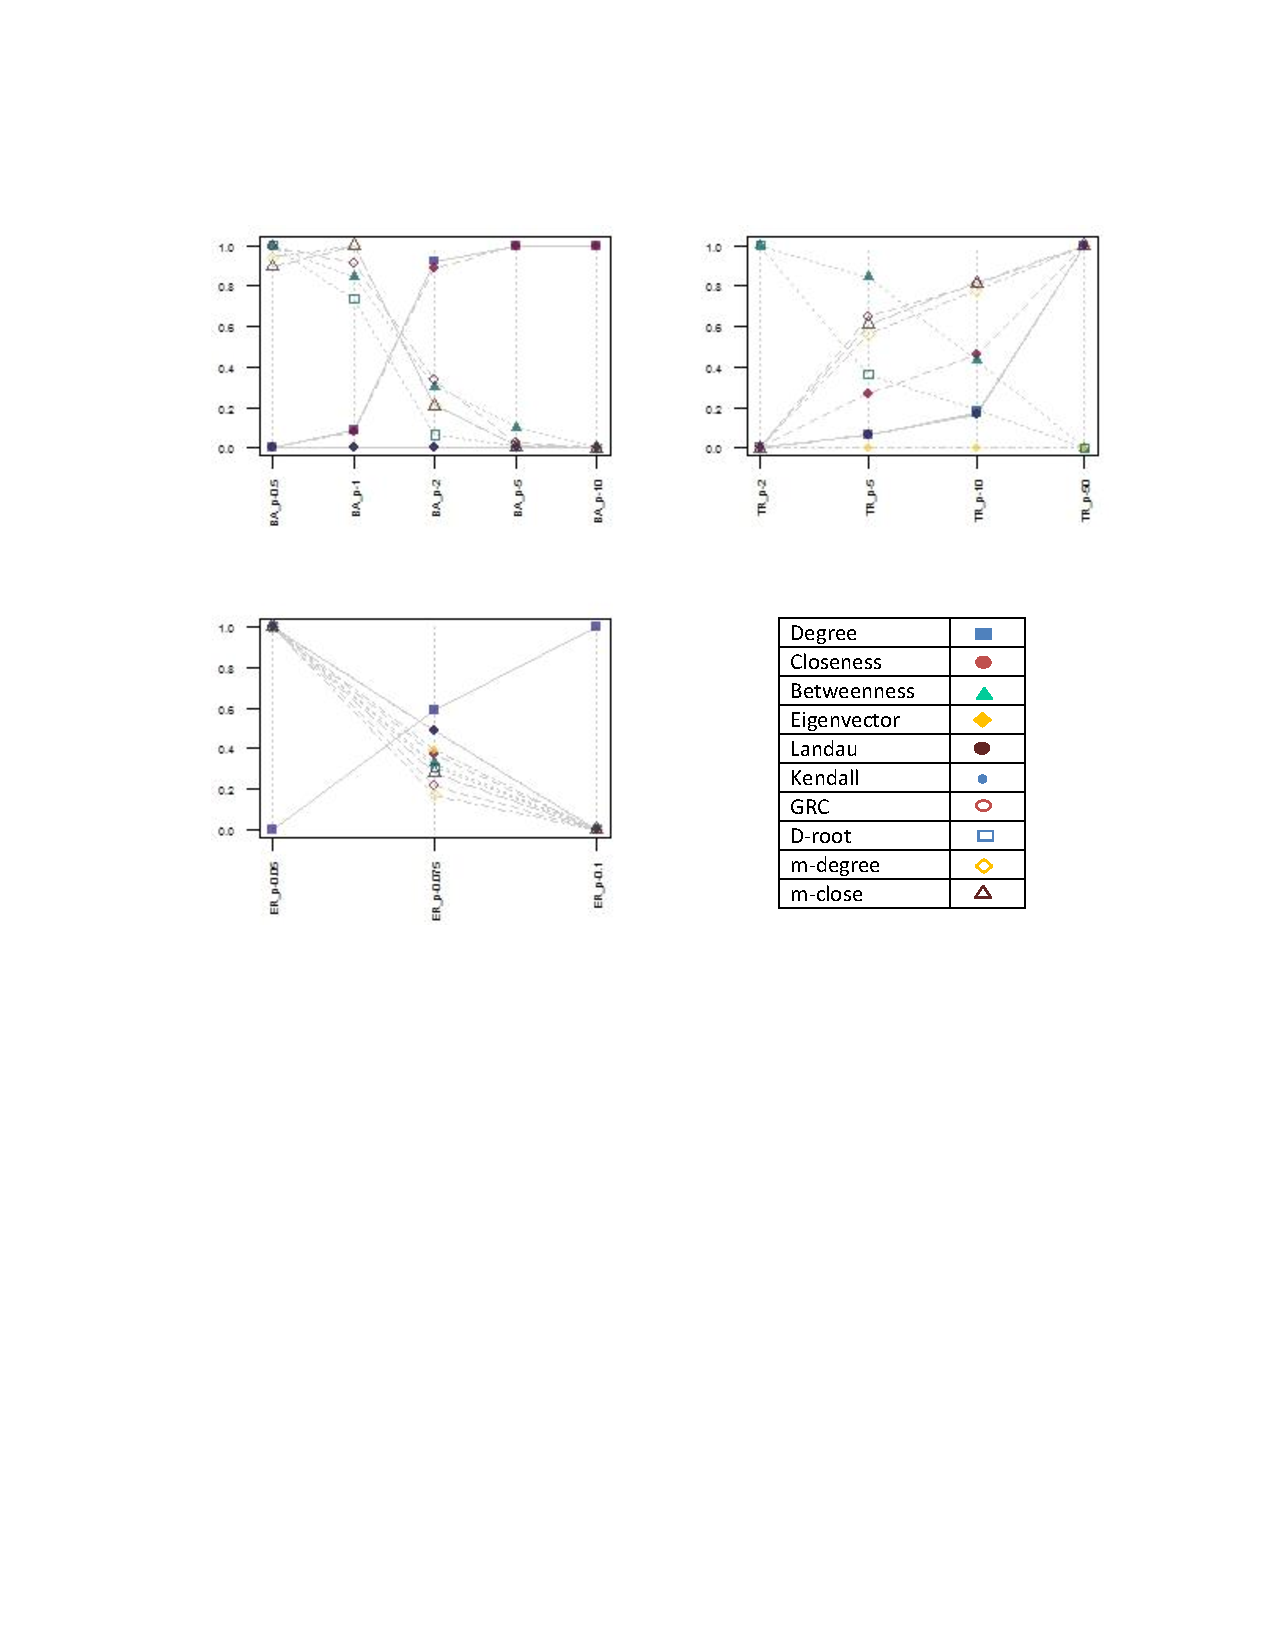
\includegraphics[width = 0.60\textwidth]{./images/Norm_Pars.pdf}
	\vspace{-5cm}
	\caption{\label{fig::Simulated Size} All figures show the average normalized global measure (denoted by the symbol in the bottom right key) by pnumber of nodes. The top left plot is for BA networks. The top right is for TR netwroks. The bottom left is for ER networks.}
	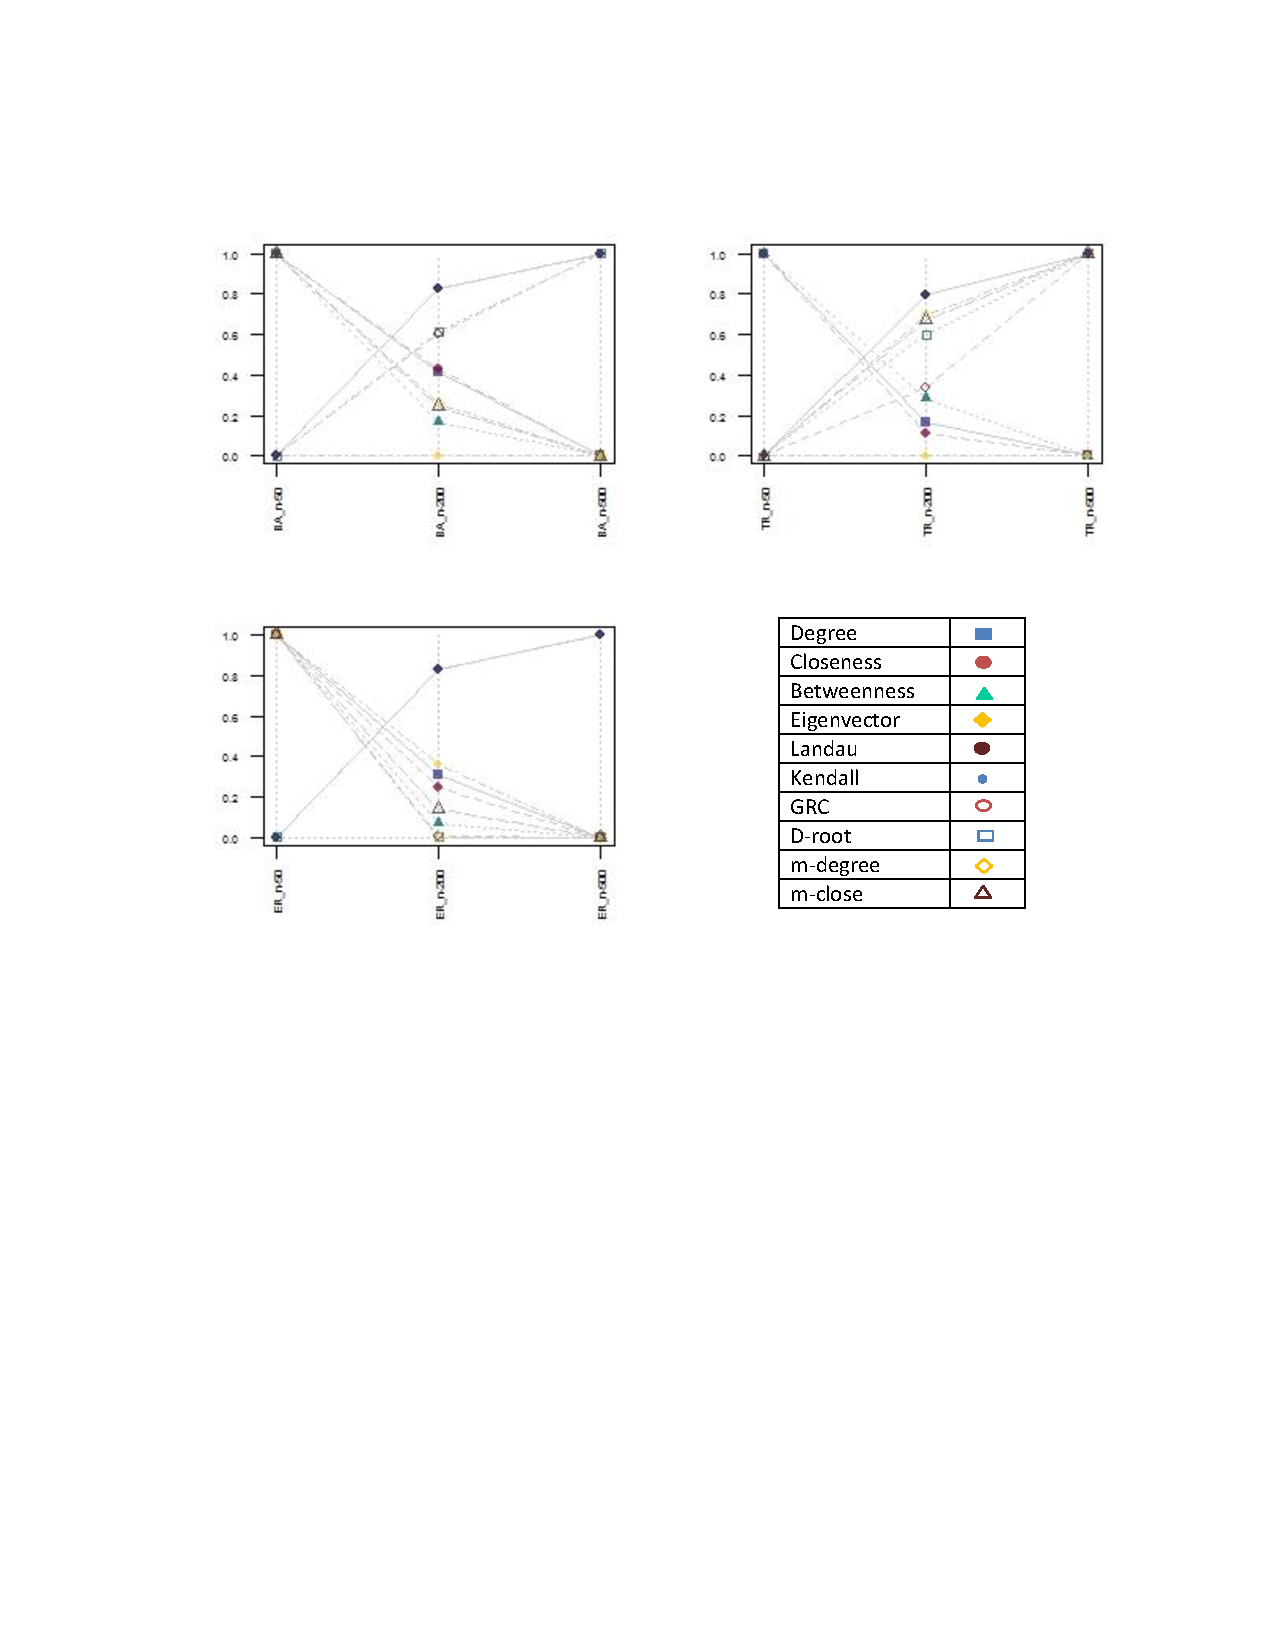
\includegraphics[width = 0.60\textwidth]{./images/Norm_Size.pdf}
	\end{center}
\end{figure}
\end{document}



%%
%% End of file `ecrc-template.tex'. 
